% =====================================================================
%  Preprint source. Compiles with `tectonic main.tex` or the standard
%  pdflatex -> bibtex -> pdflatex -> pdflatex sequence on TeX Live.
%  refs.bib is generated by scripts/fetch_bib.py; do not hand-edit it.
%  Every number in the body traces to evidence_manifest.json.
% =====================================================================

\documentclass[11pt]{article}

% ---- Page geometry ---------------------------------------------------
\usepackage[margin=1in]{geometry}

% ---- Encoding (UTF-8 source, T1 output font encoding) ---------------
\usepackage[utf8]{inputenc}
\usepackage[T1]{fontenc}

% ---- Math ------------------------------------------------------------
\usepackage{amsmath}
\usepackage{amssymb}

% ---- Graphics & tables ----------------------------------------------
\usepackage{graphicx}
\usepackage{booktabs}

% ---- Captions & colour ----------------------------------------------
\usepackage{caption}
\usepackage{xcolor}

% ---- Bibliography (numeric, author-year-capable plainnat) -----------
\usepackage[numbers]{natbib}

% ---- Hyperlinks (load late, before cleveref-style packages) ---------
\usepackage{hyperref}

% =====================================================================
%  Title / author / date macros.
% =====================================================================
\newcommand{\paperTitle}{Reproduce, Then Attribute: A Controlled Study of the
LLM Training Lifecycle on a Bit-Exact Qwen3-0.6B Reproduction}
\newcommand{\paperTitlePlain}{Reproduce, Then Attribute}
\newcommand{\paperAuthor}{Yash Bishnoi}
\newcommand{\paperDate}{\today\\[4pt]\normalsize
\url{https://github.com/yashb98/BuildFromScratch}}

\hypersetup{
  colorlinks=true,
  linkcolor=black,
  citecolor=black,
  urlcolor=blue,
  pdftitle={\paperTitlePlain},
  pdfauthor={\paperAuthor}
}

\title{\paperTitle}
\author{\paperAuthor}
\date{\paperDate}

\begin{document}

\maketitle

% ---- Abstract --------------------------------------------------------
\begin{abstract}
Published improvements to language-model training rarely arrive with
attribution: gains are reported for bundles of changes, at loosely matched
compute, often from single runs, so a reader learns that a recipe won without
learning why. Small-scale reproductions, where controlled re-testing is
affordable, are rarely held to a controlled standard. This paper carries a
bit-exact reproduction of Qwen3-0.6B (fp32 max
$|\Delta\mathrm{logits}| = 0.0$ against the reference on the recorded probe)
through the full training lifecycle -- pre-training, data composition,
mid-training, supervised fine-tuning, and reinforcement learning with
verifiable rewards -- on a single GB10 machine, admitting a comparison only
when exactly one variable differs, training FLOPs match within 5\%, and the
effect is a paired three-seed bits-per-byte (BPB) delta with a 95\% confidence
interval on two corpora. Under these gates, a modernization bundle's
single-run, in-loop $-17.9\%$ validation-perplexity headline decomposes into
three individually significant architecture effects plus an early-training
optimizer effect, while its schedule and z-loss axes contribute nothing
measurable; and a premium-data anneal improves code BPB by $+0.2716$ (95\% CI
$[+0.2641, +0.2792]$, 3 seeds, paired) over an iso-token control that absorbs
the learning-rate confound. Three nulls are reported at the same standard: SFT
response-masking does not separate from its iso-FLOP control; GRPO at 0.6B
confirms a pre-registered null against a random-reward gate (single seed,
directional by design); and context extension is gated off by a step-0
diagnostic. The same gates caught the project's own errors, including an
in-loop 0.68-perplexity ``win'' that collapsed to $+0.009$ on a fixed held-out
set.

\end{abstract}

% ---- Body ------------------------------------------------------------
\section{Introduction}\label{sec:intro}

Training reports for open language models have become admirably detailed, yet
their evidentiary unit remains the bundle: a recipe of architecture,
optimizer, schedule, and data changes is evaluated as a whole, at whatever
compute each configuration happened to consume, often from a single run. When
the bundle wins, the reader learns that it won -- not which component carried
the effect, whether the gain clears seed noise, or whether it would survive a
compute-matched control \citep{hoffmann2022training}. Adopters then inherit
every cost of the recipe -- an optimizer's throughput overhead, a data
pipeline's engineering -- without knowing which of those costs buys anything.
The gap is widest exactly where closing it would be cheapest: reproductions of
small models are common, but they typically stop at matching weights or loss
curves, and controlled re-tests of published components -- one variable,
matched FLOPs, multiple seeds -- remain rare.

This paper works in that gap by doing both halves in sequence: reproduce
first, attribute second. The substrate is a single-file reproduction of
Qwen3-0.6B-Base \citep{yang2025qwen3}, verified against the released weights
at fp32 max $|\Delta\mathrm{logits}| = 0.0$ with argmax agreement on the
recorded probe (Table~\ref{tab:repro}), so that every subsequent effect is
measured on an implementation whose fidelity is a checked gate rather than an
assumption. From that substrate the study walks the training lifecycle in
order -- pre-training attribution, data composition, mid-training, supervised
fine-tuning (SFT), and reinforcement learning with verifiable rewards (RLVR)
-- and holds every stage to one standard of evidence: a single-variable diff
at iso-FLOP (matched within 5\%), three paired seeds per arm, bits-per-byte
(BPB) deltas with 95\% confidence intervals on two corpora, and versioned
evaluation suites (Section~\ref{sec:method}).

The entire study ran on one NVIDIA GB10 with a unified CPU--GPU memory pool of
$\approx$119~GB. That constraint sets the scale honestly: the faithful base
consumed 1.19B FineWeb-Edu tokens \citep{penedo2024fineweb} -- roughly 2
tokens per parameter, far below compute-optimal
\citep{hoffmann2022training} -- and the ablation cells range from 42M to 151M
tokens per seed (Table~\ref{tab:arms}). The consequence is stated once here
and repeated wherever it matters: every effect in this paper is a fixed-budget
attribution at 596M parameters, and none is a scaling claim. What the small
scale buys in exchange is the ability to afford real controls -- re-running an
entire comparison across three seeds costs hours, not weeks -- and an
autonomous, contract-governed research loop executed the experiments
unattended, with human gates on irreversible actions
(Section~\ref{sec:method}).

The outcome is two attributed wins, three honest nulls, and a catalogue of the
project's own caught errors. The specific contributions are:

\begin{itemize}
\item \textbf{Bit-exact reproduction as a verification gate
(Section~\ref{sec:repro}).} The Qwen3-0.6B-Base reproduction (596,049,920
parameters) matches the HuggingFace reference implementation at fp32 max
$|\Delta\mathrm{logits}| = 0.0$; a second reproduction, SmolLM2-135M
(134,515,008 parameters), passes the same gate and calibrates how much logit
noise device kernels alone introduce (Table~\ref{tab:repro}). A faithful
baseline trained on the 1.19B-token budget lands at 2.14$\times$ the original
model's perplexity at $\approx$30,000$\times$ less data -- reported
descriptively only, as a single-run, in-loop measurement
(Figure~\ref{fig:repro-gap}).

\item \textbf{An evidence-gating methodology that decides what a number may be
called (Section~\ref{sec:method}).} Comparisons are admitted only under a
single-variable diff at iso-FLOP; effects are paired three-seed BPB deltas
with 95\% confidence intervals on two corpora, scored by version-stamped
suites; a missing required evaluation or a single-seed design caps a verdict
at directional; and pre-registered expectations bind in both directions --
including against the authors, as when a pre-registered English null was
violated and reported as such (Table~\ref{tab:midtrain}).

\item \textbf{A de-confounded modernization bundle
(Section~\ref{sec:pretrain}).} The motivating result -- an IMU-1-derived
bundle \citep{grigorev2026imu} beating the faithful baseline by 17.9\% in-loop
validation perplexity at matched 1.19B-token budgets, a single run, not
suite-stamped (Figure~\ref{fig:ppl-curves}) -- is decomposed by re-testing its
axes one variable at a time. Only the architecture axis is significant
($+0.1179$ BPB on WikiText-2, 95\% CI $[+0.1005, +0.1354]$, 3 seeds, paired,
text-lm-v2), and it splits into three individually significant components:
value residuals $+0.0355$ $[+0.0116, +0.0594]$, LayerNorm scaling $+0.0337$
$[+0.0175, +0.0498]$, and head gating $+0.0256$ $[+0.0125, +0.0386]$
(Table~\ref{tab:attrib}, Figure~\ref{fig:deconfound}). The WSD schedule and
z-loss axes contribute nothing measurable. The NorMuon optimizer
\citep{li2025normuon} is isolated separately as a large early-training
optimization-speed effect ($+0.4743$ BPB at 42M tokens per arm, 95\% CI
$[+0.4435, +0.5052]$), defended by a matched-config AdamW learning-rate sweep
and explicitly scoped to its budget, not to scale (Table~\ref{tab:attrib}).

\item \textbf{Single-variable data and mid-training effects
(Sections~\ref{sec:data} and~\ref{sec:midtrain}).} At matched tokens, a
dclm-edu corpus \citep{li2024datacomp} improves code BPB over FineWeb-Edu by
$+0.7034$ (95\% CI $[+0.6639, +0.7430]$, 3 seeds, paired, text-lm-v2) -- the
largest single effect in the study -- and a sequence-preserving 50/50 mix
retains 83.9\% of that code win while preserving English
(Table~\ref{tab:data}). A premium-mix anneal then beats an iso-token
continued-pretraining control on code by $+0.2716$ BPB (95\% CI
$[+0.2641, +0.2792]$, 3 seeds, paired) while the control barely moves off the
base, so the learning-rate-decay-plus-extra-tokens confound is absorbed by
construction (Table~\ref{tab:midtrain}).

\item \textbf{Negative results at the same standard as the wins
(Sections~\ref{sec:sft} and~\ref{sec:rlvr}).} Response-masked SFT does not
separate from an iso-FLOP continued-pretraining control on a fixed held-out
set: the masked comparison and a tokenizer-free full-sequence cross-check
disagree in sign, so the verdict of record is directional
(Table~\ref{tab:sft}). GRPO at 0.6B confirms a pre-registered null
\citep{yue2025does}: it beats neither its SFT floor nor a mandatory
random-reward gate \citep{shao2025spurious}, with training reward flat at
$\approx$0.9\% throughout (Table~\ref{tab:rlvr}, Figure~\ref{fig:rlvr};
math-acc-v1, single seed, directional by design). Context extension was gated
off at step 0 by a pre-registered passkey threshold the base failed at its own
trained window (Section~\ref{sec:midtrain}).

\item \textbf{A failure catalogue (Section~\ref{sec:failures}).} Seven
file-backed failures are reported as symptom, detection, root cause, fix, and
guard -- including an in-loop 0.68-perplexity SFT ``win'' that collapsed to
$+0.009$ once re-scored on one fixed held-out token set
(Figure~\ref{fig:sft-confound}), and a token-level shuffle bug flagged because
its result was physically implausible. None of the seven was caught by
re-reading prose; all were caught by the same mechanical gates that validate
the positive results.
\end{itemize}

The remainder of the paper is organized as follows.
Section~\ref{sec:related} situates the study among open small-model reports,
matched-compute practice, and the RLVR debate. Section~\ref{sec:method}
defines the evidence gates and verdict semantics; Section~\ref{sec:setup}
specifies the model, data, hardware, and evaluation protocol.
Section~\ref{sec:repro} establishes the verification gate and the faithful
baseline. Sections~\ref{sec:pretrain} through~\ref{sec:rlvr} then present the
lifecycle results in training order -- pre-training attribution, data
composition, mid-training, SFT, and RLVR -- and
Section~\ref{sec:failures} collects what the gates caught. The paper closes
with discussion and limitations, a reproducibility statement
(Section~\ref{sec:repro-statement}), and broader impacts
(Section~\ref{sec:impacts}).
        % 1. Introduction + contributions
\section{Related Work}\label{sec:related}

\paragraph{Open small-LM training reports and reproductions.}
Small language models increasingly ship with detailed training documentation. Qwen3 releases open weights down to 0.6B parameters \citep{yang2025qwen3}; SmolLM2 documents a data-centric, multi-stage recipe at 1.7B and releases its curated datasets \citep{allal2025smollm2}; OLMo~2 releases weights, data, code, recipes, and intermediate checkpoints \citep{olmo20242}; and MiniCPM develops small-model training strategies systematically \citep{hu2024minicpm}. Closest to our setting, IMU-1 trains a 430M-parameter model with a bundle of modernizations -- the NorMuon optimizer, QK-norm, per-head gating, value residuals, and LayerNorm scaling, among others -- and reports approaching the benchmark performance of models trained on far more data, with per-component ablations \citep{grigorev2026imu}. On the data side, FineWeb documents ablation-driven web curation \citep{penedo2024fineweb}, and DataComp-LM provides a controlled testbed in which model-based filtering emerges as the key lever \citep{li2024datacomp}; our data-composition experiment places a dclm-edu arm against a FineWeb-Edu control at matched tokens (Table~\ref{tab:data}). These reports evaluate recipes as bundles at production scale. We work in the opposite direction: reproduce one released model bit-exactly (Table~\ref{tab:repro}), then re-test which published components survive single-variable, iso-FLOP, multi-seed attribution on a different base, data pipeline, and budget (Figure~\ref{fig:deconfound}).

\paragraph{Optimizers and baseline-tuning discipline.}
NorMuon adds neuron-wise normalization to Muon's orthogonalized updates and reports efficiency gains over both Adam and Muon at the 1.1B scale \citep{li2025normuon}, with AdamW \citep{loshchilov2017decoupled} the default comparator. Because optimizer wins are routinely attributed to undertuned baselines, our NorMuon-vs-AdamW comparison (+0.4743 BPB on wikitext-2, 95\% CI [+0.4435, +0.5052], 3 seeds, paired, iso-FLOP at 42M tokens per arm, text-lm-v2; Table~\ref{tab:attrib}) carries a matched-configuration AdamW learning-rate sweep whose entire spread is roughly one tenth of the gap in Table~\ref{tab:attrib}, and we scope the result as an early-training optimization-speed signal at one architecture and one budget, not a claim about behavior at scale.

\paragraph{Compute-optimal scaling and matched-compute comparison.}
Chinchilla showed that at fixed compute, parameters and training tokens should scale together, and it compared models at an equalized compute budget \citep{hoffmann2022training}; we follow the FLOP-accounting conventions of \citet{chowdhery2022palm}. This study inherits the matched-compute discipline rather than extending it: every comparison varies exactly one factor with training FLOPs matched within 5\%, and all budgets sit far below compute-optimal (the base run is $\approx$2 tokens per parameter; Table~\ref{tab:arms}), so effects are reported as fixed-budget attributions, never scaling laws.

\paragraph{Mid-training, annealing, and long-context evaluation.}
MiniCPM's warmup-stable-decay schedule frames the decay phase as a vehicle for continued training and domain adaptation \citep{hu2024minicpm}; OLMo~2 applies a dedicated late-stage mixture during annealing \citep{olmo20242}, and SmolLM2 rebalances its mixture across stages \citep{allal2025smollm2}. Such reports motivate premium-data anneals but seldom isolate the data effect from the learning-rate decay that accompanies it. Our anneal therefore carries an iso-token control under the identical cooldown: the control barely moves off the base, while the premium mix improves code BPB by +0.2716 (95\% CI [+0.2641, +0.2792], 3 seeds, paired, 150.7M tokens per cell, text-lm-v2; Table~\ref{tab:midtrain}). For long context we adopt the passkey retrieval probe of \citet{mohtashami2023landmark} as a per-rung accuracy ladder with Wilson intervals (ecl-ladder-v1; Figure~\ref{fig:ecl-ladder}), consistent in spirit with RULER's finding that claimed context lengths overstate effective ones \citep{hsieh2024ruler}.

\paragraph{RLVR skepticism at small scale.}
Recent work questions how much reinforcement learning with verifiable rewards adds beyond the base model. \citet{yue2025does} find via large-$k$ pass@$k$ that base models match or exceed their RLVR-trained counterparts, concluding that RLVR sharpens what the base model already contains rather than expanding it; \citet{shao2025spurious} show that randomly assigned rewards produce large MATH-500 gains on Qwen2.5-Math models specifically and urge validation across model families, which motivates our mandatory random-reward control on a Qwen-lineage base; \citet{liu2025understanding} identify optimization biases in GRPO and propose the unbiased Dr.~GRPO variant we adopt; and DAPO documents the system-level techniques needed to make large-scale RLVR reproducible \citep{yu2025dapo}. VibeThinker-3B argues the optimistic case, reporting benchmark results at 3B parameters that it claims rival far larger systems \citep{xu2026vibethinker}. We contribute a pre-registered small-scale data point: Dr.~GRPO with DAPO-style group filtering on our 0.6B base beats neither its SFT floor nor the random-reward gate on GSM8K \citep{cobbe2021training} or MATH-500 levels 1--3 \citep{hendrycks2021measuring}, with training reward flat at $\approx$0.9\% (Table~\ref{tab:rlvr}, Figure~\ref{fig:rlvr}; math-acc-v1, n=1 seed, directional by design), scored under the pass@$k$ protocol of \citet{chen2021evaluating} with Wilson intervals.

\paragraph{Positioning.}
This paper introduces no new training technique. Its contribution is single-variable, iso-FLOP, multi-seed attribution of published techniques at reproduction scale on one machine, anchored by a bit-exact reproduction, together with negative results reported at the same standard as wins: SFT response-masking that does not separate from its iso-FLOP control (Table~\ref{tab:sft}), the pre-registered GRPO null (Table~\ref{tab:rlvr}), and a context-extension direction gated off by a step-0 diagnostic.
             % 2. Related work
\section{Evidence-Gated Methodology}\label{sec:method}

This study is as much about method as about results. Every experiment was
executed by an autonomous research loop on a single machine, governed by
machine-checkable contracts that decide what may launch, what may be measured,
and what a number is allowed to be called. The notation and verdict semantics
defined here are used by all results sections.

\subsection{The Unit of Claim}

The atomic claim of this paper is a \emph{paired across-seed bits-per-byte
(BPB) delta with a 95\% confidence interval, reported on at least two corpora,
under a single-variable diff at iso-FLOP, scored by a versioned harness against
a measured noise floor}. Each ingredient is defined below.

\textbf{Metric.} For a model $m$ and a fixed evaluation corpus $C$ of byte
length $B(C)$, tokenized by $m$'s own tokenizer into $x_1,\dots,x_N$,
\begin{equation}
\mathrm{BPB}(m,C) \;=\; \frac{1}{B(C)} \sum_{t=1}^{N} -\log_2 p_m\!\left(x_t \mid x_{<t}\right).
\end{equation}
Because the denominator is a property of the raw text rather than of any
tokenization, BPB remains comparable when tokenizers differ and across corpora,
unlike per-token perplexity. The harness scores fixed windows of 204{,}600
tokens per corpus over 869{,}710 bytes of WikiText-2 and 843{,}643 bytes of
held-out Python code, at pinned dataset revisions, with 13-gram decontamination
against training data; per-checkpoint perplexities and noise floors on these
corpora appear in Table~\ref{tab:arms}. Effects must be reported on both
corpora: $\Delta_c = \mathrm{BPB}_{\mathrm{base}}(c) -
\mathrm{BPB}_{\mathrm{treat}}(c)$, positive meaning improvement.

\textbf{Single variable at iso-FLOP.} Two arms compare only if exactly one
variable differs \emph{and} their training FLOPs, under the
$6N + 12 \cdot L \cdot H \cdot Q \cdot T$ accounting of \citet{chowdhery2022palm},
match within 5\%; comparisons at unequal compute conflate the variable with
budget \citep{hoffmann2022training}. Token-matched is not FLOP-matched when the
architecture or optimizer cost changes, so the check is computed, not assumed,
and recorded with each run (the largest recorded mismatch among the pretraining
comparisons is a FLOPs-per-token ratio of 1.00043; Table~\ref{tab:attrib}).
Every comparison states its matched budget in tokens and steps
(Table~\ref{tab:hparams}).

\textbf{Paired seed test.} Both arms train the identical seed set
$\{0,1,2\}$, varying initialization and data order. The effect is the
difference of arm means with a Student-$t$ 95\% interval,
$\Delta_c \pm t_{0.975,\nu}\sqrt{\mathrm{SEM}_b^2+\mathrm{SEM}_t^2}$, where
$\nu$ is the Welch--Satterthwaite degrees of freedom floored to an integer
(conservative at $n{=}3$, where a normal quantile would be too narrow). A delta
is \emph{significant} only if the entire interval lies on the improving side of
zero. A corpus-subsample noise floor -- the spread of the baseline checkpoint
over three disjoint evaluation subsamples -- is retained as a secondary check;
deltas below it are labeled not significant. The floors themselves motivate the
design: on this suite the code-corpus perplexity floor is large
(Table~\ref{tab:arms}), so single-checkpoint perplexity gaps on code are close
to meaningless, whereas across-seed BPB intervals are not. Results are quoted
as $+X$ BPB (95\% CI $[\mathrm{lo},\mathrm{hi}]$, 3 seeds, paired).

\textbf{Versioned harness.} Cross-run comparable numbers come only from the
evaluation harness, which stamps a suite version into every result:
(text-lm-v2) for the BPB/perplexity suite, (math-acc-v1) for the pinned math
answer-extractor and verifier, (ecl-ladder-v1) for the passkey context ladder.
Any suite change bumps the version, so numbers with different stamps are never
differenced. Perplexities printed by the training loop are labeled in-loop
validation perplexity, single run, and are advisory only. This distinction is
load-bearing: an in-loop 0.68-perplexity SFT ``win'' collapsed to $+0.009$
(95\% CI $[0.0045, 0.0139]$) once re-scored on one fixed held-out token set
(Figure~\ref{fig:sft-confound}).

\subsection{Claim Classes and Verdict Caps}

Verdicts take the values \emph{win}, \emph{loss}, \emph{inconclusive}, and
\emph{directional}. Every run carries a lifecycle stage (data, architecture,
mid-training, sft, rlvr, \dots), and a per-stage registry names the required
(HARD) evaluation battery for that stage. A missing HARD item forces the
verdict to directional regardless of the point estimate -- completeness gates
significance, not the reverse. A single-seed run is never significance-testable
and is likewise capped at directional; the RLVR cohort was run at one seed by
pre-registered design and carries exactly this cap (Table~\ref{tab:rlvr}).
Near-chance downstream results are reported with Wilson intervals as no-signal,
never as wins, with pass@$k$ computed by the unbiased estimator of
\citet{chen2021evaluating}.

\subsection{Control Reuse and Pre-Registration}

Baseline checkpoints are reused across experiments as symlinks and re-scored
in-cohort, so every number in a comparison comes from the same evaluation pass
of the same harness version: the architecture sub-drill reuses the de-confound
baselines (Table~\ref{tab:attrib}), and the data-mix study reuses the dclm-edu
arm (Table~\ref{tab:data}). Expected outcomes are written down before launch
and bind in both directions. The RLVR plan, written 2026-07-01 before the
2026-07-02 launch, predicted a null at this scale
\citep{yue2025does} and mandated a random-reward control for Qwen-lineage
models \citep{shao2025spurious}; the null was confirmed
(Figure~\ref{fig:rlvr}). The mid-training anneal pre-registered an expected
English null that the data violated -- $+0.0157$ BPB (95\% CI
$[+0.0140, +0.0174]$, 3 seeds, paired; Table~\ref{tab:midtrain}) -- and the
violation is reported as exploratory rather than promoted to a claim.

\subsection{Launch Evidence and the Ledger}

No budgeted GPU run starts until its evidence is recorded: a literature-sourced
token budget, the arm~$\times$~seed plan, the confound check, a measured
throughput probe with a derived ETA, and a passing smoke test that executes the
exact training script for one step on a tiny batch and asserts a finite,
descending loss, a checkpoint save-then-reload round trip, and exit code zero.
The ledger is the append-only truth store: a single programmatic interface with
atomic writes records techniques, runs, verdicts, suite stamps, and costs, and
is the deduplication authority for what has already been tried. A resumable
state machine executes the stages unattended -- preflight, scan, selection,
briefing, data preparation, launch, evaluation, verdict -- and always ends by
writing a digest, while irreversible actions (new model builds, compute spend,
publication) remain human-gated.

\subsection{Safety Envelope}

All training ran on one NVIDIA GB10 with a unified CPU+GPU memory pool of
$\approx$119~GB and no separate VRAM; over-allocation invokes the kernel
OOM-killer and can take down the machine, so safety limits are part of the
method. Three constraints apply to every job: (i) a per-process allocator guard
caps GPU memory at a 0.85 fraction of the pool and is imported before the
framework in every script; (ii) an independent watchdog process kills any
unattended trainer at a 0.80 pool fraction -- strictly below the guard, so the
watchdog fires first -- and only one trainer may run at a time; (iii)
cross-entropy over the 151{,}936-token vocabulary is computed in chunked fp32,
never materializing the full sequence-by-vocabulary logit matrix. Throughput
and MFU figures are reported as approximate throughout, because the device peak
for this hardware is an estimate.
         % 3. Evidence-gated methodology (contracts, gates, loop)
\section{Experimental Setup}\label{sec:setup}

\paragraph{Model.}
All experiments run on our from-scratch reproduction of Qwen3-0.6B-Base
\citep{yang2025qwen3}: a pre-norm, decoder-only transformer
\citep{vaswani2017attention} with 28 layers and hidden size 1{,}024.
Attention is grouped-query \citep{ainslie2023gqa} with 16 query heads and
8 key--value heads at an explicit head dimension of 128, set independently
in the configuration (it is not hidden size divided by head count, which
would give 64). Each block applies RMSNorm \citep{zhang2019root} with
$\epsilon = 10^{-6}$ before attention and before a SwiGLU feed-forward
network \citep{shazeer2020glu} of intermediate size 3{,}072; Qwen3
additionally normalizes queries and keys per head (QK-norm, an RMSNorm
over the 128-dimensional head axis) before rotary position embeddings
\citep{su2021roformer} with base $\theta = 10^{6}$ and positions up to
40{,}960. All projections are bias-free, and the input embedding is tied
to the output head over a 151{,}936-entry vocabulary. Recomputed from
this configuration, the model has exactly 596{,}049{,}920 parameters:
28 blocks of 15{,}730{,}944 each, a tied embedding matrix of
155{,}582{,}464, and a 1{,}024-parameter final norm
(Table~\ref{tab:repro}). A second reproduction, SmolLM2-135M
\citep{allal2025smollm2} with 134{,}515{,}008 parameters, shows that the
verification protocol is not specific to one model family
(Table~\ref{tab:repro}).

\paragraph{Tokenizer.}
We use the Qwen3 byte-level BPE tokenizer with vocabulary size
151{,}936. Every perplexity in this paper is computed with the model's
own tokenizer; cross-tokenizer perplexity comparisons are never made.
Cross-corpus effects are reported in bits per byte (BPB), which
normalizes cross-entropy by the UTF-8 byte count of the scored text and
is tokenizer-independent.

\paragraph{Data.}
The pre-training corpus is FineWeb-Edu \citep{penedo2024fineweb}
(\texttt{sample-10BT}), streamed and tokenized on the fly. The baseline
consumes 1{,}189{,}478{,}400 training tokens (18{,}150 steps at
65{,}536 tokens per step; Table~\ref{tab:hparams}), approximately
2 tokens per parameter -- deliberately far below the compute-optimal
ratio \citep{hoffmann2022training}, since the study optimizes for
controlled comparisons rather than absolute quality. A held-out
validation slice of 300{,}012 tokens is document-disjoint from training
via a seeded hash split and screened by 13-gram overlap decontamination
(0 of 451 validation documents dropped); the in-loop evaluator scores
50 windows of 4{,}096 tokens (204{,}800 tokens) on this slice. The
data-composition experiments add a dclm-edu slice \citep{li2024datacomp}
of 150{,}107{,}480 training tokens, pinned by content hash
(\texttt{dbad8ad7}) and decontaminated with the same 13-gram screen
against both evaluation corpora (0 documents dropped). Supervised
fine-tuning uses OpenR1-Math-220k pairs totalling 125{,}000{,}592
tokens. The GRPO prompt set (\texttt{grpo-math-prompts-v1}) contains
7{,}471 GSM8K and 3{,}490 MATH level 1--3 training prompts after
dropping 14 prompts that overlapped the evaluation sets at the 13-gram
level; 7 prompts overlapping the SFT set were flagged and kept. The math
evaluation sets themselves (\texttt{math-eval-v1}) are decontaminated
against all 35{,}924 OpenR1 SFT problems: 0 of 1{,}319 GSM8K test items
and 0 of 500 MATH-500 items are flagged.

\paragraph{Hardware.}
Everything runs on one NVIDIA GB10 (Grace Blackwell) workstation whose
CPU and GPU share a single $\approx$119 GB unified-memory pool with no
separate VRAM. Training uses bfloat16 with \texttt{torch.compile} at
sequence length 4{,}096; cross-entropy over the 151{,}936-entry
vocabulary is computed in fp32 chunks, since materializing the full fp32
logit matrix at this vocabulary size is infeasible in the shared pool.
A 50-step probe measured 7{,}167.4 tokens/s compiled versus 3{,}787.5
uncompiled (a 1.89$\times$ speedup), and the full baseline run sustained
7{,}444--7{,}482 tokens/s at a flat 52.4 GB peak memory, completing in
2{,}663.1 minutes. FLOP accounting follows the PaLM convention
\citep{chowdhery2022palm}. Because the GB10's peak throughput is an
estimate rather than a published figure, model FLOPs utilization is
reported as approximate only and never as an exact number.

\paragraph{Evaluation protocol.}
Three versioned suites produce every cross-run comparable number, and
each such number carries its suite stamp. (i) \textbf{text-lm-v2}:
perplexity and BPB on the wikitext-2-raw-v1 validation split and
codeparrot-clean-valid, both at pinned dataset revisions
(\texttt{b08601e}, \texttt{4db92d2}), scoring 204{,}600 tokens per
corpus per cell. The harness measures a per-corpus noise floor on the
baseline checkpoint: 1.304 PPL (3.73\% relative) on wikitext-2 but
280.6 PPL (68.2\% relative) on the code corpus (Table~\ref{tab:arms}).
Code-perplexity orderings are therefore always quoted with this caveat,
and comparative effects are instead reported as BPB improvements with
paired 3-seed 95\% confidence intervals, where seeds vary initialization
and data order; deltas below the floor or with an interval crossing zero
are labeled not significant. (ii) \textbf{math-acc-v1}: a pinned answer
extractor and verifier over GSM8K \citep{cobbe2021training} and MATH-500
levels 1--3 \citep{hendrycks2021measuring}, with pass@$k$ computed by
the unbiased estimator of \citet{chen2021evaluating} and Wilson 95\%
intervals for pass@1, under a fixed sampling band (8 samples per item,
temperature 0.8, 256 new tokens, fixed band seed) on 100 GSM8K and
50 MATH-500 items. (iii) \textbf{ecl-ladder-v1}: passkey retrieval
\citep{mohtashami2023landmark} across context rungs 512--8{,}192 at
depths 0.1--0.9, with 40 probes per rung per cell and Wilson intervals,
an effective-context-length measurement in the spirit of RULER
\citep{hsieh2024ruler}. Trainer-internal perplexities are labeled
throughout as in-loop validation perplexity, single run, not
suite-stamped, and are advisory only. Comparative arms are
single-variable and iso-FLOP by construction: two arms are compared only
if exactly one variable differs and their training FLOPs match within
5\%, with matched token and step budgets stated for every comparison.

\paragraph{Hyperparameters.}
Table~\ref{tab:hparams} consolidates the per-stage hyperparameters --
optimizer, learning-rate schedule, warmup, weight decay, batch shape,
token and step budgets, and seeds -- with each value flagged as reported
in its source paper, inferred from a published band, or chosen by us
where no published value exists at this scale. AdamW
\citep{loshchilov2017decoupled} is the optimizer at every stage except
the treatment arm of the optimizer A/B itself.

% ---------------------------------------------------------------------
% tab_hparams.tex -- per-stage hyperparameters for every experiment
% stage in the paper. Every value is transcribed from the run's
% c5_evidence.json recipe, the trainer's argparse defaults, or the
% args/start line of the on-disk training log.
% Provenance flags: R = reported in the cited source paper;
% I = inferred (source gives a band, we picked a point);
% C = chosen by us (no published value at this scale/budget).
% ASCII only; requires only booktabs.
% ---------------------------------------------------------------------
\providecommand{\hpR}{\textsuperscript{R}}
\providecommand{\hpI}{\textsuperscript{I}}
\providecommand{\hpC}{\textsuperscript{C}}

\begin{table}[t]
\centering
\caption{Per-stage training hyperparameters. Superscripts flag
provenance: \hpR{} reported in the source paper (Qwen3 technical
report LR shape; VibeThinker SFT stage-1; GRPO/DAPO/Dr.GRPO),
\hpI{} inferred from a band in the source, \hpC{} chosen by us (no
published value at this scale). Shared unless stated: AdamW betas
$(0.9,0.95)$, eps $10^{-8}$, grad-clip 1.0, bf16, seq.\ len.\ 4096,
chunked fp32 cross-entropy, one GB10 GPU; all part-(a) stages use
65{,}536 tok/step (micro-batch 4 $\times$ grad-accum 4)\hpC. Each run
directory records its full recipe in \texttt{c5\_evidence.json} before
launch (contract C5); values are cross-checked against the
\texttt{args} lines of the training logs. The optimizer A/B also ran a
matched-config AdamW LR sweep $\{1.7,2.4,3.5,4.8\}\times10^{-3}$ (n=1
off-baseline). GRPO Phase 2 is n=1 by design (verdict capped at
directional).}
\label{tab:hparams}
\footnotesize
\setlength{\tabcolsep}{3.5pt}
\renewcommand{\arraystretch}{1.05}

% ---- (a) Pre-training and mid-training stages ------------------------
\begin{tabular}{@{}lp{2.0cm}p{2.2cm}p{2.6cm}p{2.3cm}p{2.2cm}@{}}
\toprule
 & \textbf{Faithful 2TPP} & \textbf{Optimizer A/B} & \textbf{De-confound P1/P2} & \textbf{Data cells} & \textbf{Mid-train anneal} \\
 & (06-08) & (06-16) & (06-18 / 06-21) & (06-24 / 06-26) & (06-30) \\
\midrule
Init            & random & random & random & random & 2TPP ckpt \\
Data            & FineWeb-Edu\hpC & FineWeb-Edu\hpC & FineWeb-Edu\hpC & dclm-edu; 50/50 mix\hpC & dclm-edu, FineWeb\hpC \\
Arms            & --- & AdamW vs NorMuon-2D & +WSD, +z-loss, +arch; VR, LNS, HG & dclm; mix (ctrl reused) & 50/50 mix vs FineWeb-only \\
Optimizer       & AdamW\hpR & AdamW vs NorMuon\hpC & AdamW\hpR & AdamW\hpR & AdamW\hpR \\
LR peak $\to$ end & 2.4e-3\hpC $\to$ 3.2e-4\hpR & 2.4e-3\hpC; NM 0.011\hpC{} ($\to$ 0.1x)\hpC & 1.7e-3\hpR $\to$ 3.2e-4\hpR & 1.7e-3\hpR $\to$ 3.2e-4\hpR & 2.5e-4\hpC $\to$ 2.5e-5\hpC \\
Schedule        & cosine\hpR & cosine\hpR & cosine\hpR{} (WSD arm: WSD) & cosine\hpR & 1-sqrt decay\hpR{} (shape) \\
Warmup (steps)  & 900\hpC & 50\hpC & 100\hpC & 100\hpC & 46\hpC \\
Weight decay    & 0.01\hpR & 0.1 (2D)\hpC & 0.01\hpR & 0.01\hpR & 0.01\hpR \\
Steps (tok)/cell & 18{,}150 (1.19B, 2~TPP\hpC) & 640 (41.9M\hpC) & 2{,}000 (131M\hpC) & 2{,}000 (131M\hpC) & 2{,}300 (151M\hpC) \\
Cells (new)     & 1 & 6 & 12 / 9 & 3 / 3 & 6 \\
Seeds           & 0 & 0--2 & 0--2 & 0--2 & 0--2 \\
\bottomrule
\end{tabular}

\vspace{5pt}

% ---- (b) Post-training stages ----------------------------------------
\begin{tabular}{@{}lp{4.6cm}p{5.6cm}@{}}
\toprule
 & \textbf{SFT 3-seed} (06-27) & \textbf{GRPO Phase 2} (07-02) \\
\midrule
Init             & faithful 2TPP base (strict load) & SFT seed-0 ckpt (policy + frozen KL ref) \\
Data             & OpenR1-Math-220k pairs\hpC & grpo-math-prompts-v1: GSM8K + MATH L1--3, 2:1 mix\hpC \\
Arms             & masked SFT vs no-mask iso-FLOP control & Dr.GRPO vs random-reward vs RFT \\
Optimizer / LR   & AdamW, 5e-5\hpR $\to$ 8e-8\hpR{} cosine & AdamW, 1e-6 const.\hpI{} (RFT: 1e-5\hpI) \\
Warmup / wd      & 5\% (11 steps)\hpR{} / 0.01\hpC & none / 0.0\hpC \\
Batch            & 524{,}288 tok/step (mb 4 x ga 32 = 128 seqs\hpR) & 16 prompts x G=8 rollouts / step\hpC \\
Steps (budget)   & 238 (125M tok\hpC) & 300 (300 x 16 x 8 rollouts, cap 256 new tok\hpC) \\
Sampling         & --- & T = 0.8\hpC, no KV cache (exact re-forward) \\
Clip / KL        & --- & clip eps 0.2\hpR; k3-KL beta 3e-3\hpI \\
Reward           & --- & math-acc-v1: 1.0 / 0.1 / 0.0\hpC; random arm Bernoulli(0.5) \\
Seeds            & 0--2 & 0 (n=1, directional) \\
\bottomrule
\end{tabular}
\end{table}

               % 4. Experimental setup (arch, data, hparams, eval protocol)
\section{Bit-Exact Reproduction and the Faithful Baseline}\label{sec:repro}

Every comparison in this study is anchored to implementations that are first
verified to be exact copies of their published references. This section
documents the verification gate, the faithful small-budget baseline trained on
the verified backbone, and where that baseline sits relative to the original
released model. It makes no comparative claims beyond that descriptive
placement.

\subsection{The verification gate}

The gate is a deterministic forward-logits comparison: the official
HuggingFace weights are loaded into our from-scratch \texttt{model.py}, a
single fixed prompt (``The capital of France is'', input shape $[1,5]$) is run
in fp32, and the next-token logits are compared element-wise against the
reference implementation, with a pass threshold of
$\max|\Delta\text{logits}| < 10^{-3}$ plus argmax agreement. For our
Qwen3-0.6B reproduction~\citep{yang2025qwen3} the recorded result is not
merely within tolerance but exact: $\max|\Delta\text{logits}| = 0.0$, relative
error $0.0$, and both implementations predict token id 12095 (`` Paris'')
(Table~\ref{tab:repro}). We state the protocol's scope plainly: it is one
prompt, fp32, forward logits only -- it establishes operator-level
implementation identity under the loaded weights, not behavioral equivalence
over an input distribution. The parameter count of 596{,}049{,}920 is the
forward-calculation total of the build's architecture plan, asserted (within
1\%) by the build's unit test, rather than a field written by the verification
artifact itself.

% tab_repro.tex -- reproduction verification gate
% Sources (re-read 2026-07-06):
%   Qwen3-0.6B/builds/2026-06-08_reproduce-faithful_qwen3-0.6b/results/verify.json
%   Qwen3-0.6B/builds/2026-06-08_reproduce-faithful_qwen3-0.6b/architecture_plan.md (param total, line 60)
%   SmolLM2-134(base)/results/param_count.log, parity.log, comparison_with_hf.md
\begin{table}[t]
\centering
\small
\setlength{\tabcolsep}{4.5pt}
\begin{tabular}{@{}llrlll@{}}
\toprule
Model & HF reference & Params & $\max|\Delta\text{logits}|$ & Argmax & Device \\
\midrule
Qwen3-0.6B (ours) & \texttt{Qwen/Qwen3-0.6B-Base} & 596{,}049{,}920 & $0.0$ & match & CPU/GPU fp32 \\
SmolLM2-135M (ours) & \texttt{HuggingFaceTB/SmolLM2-135M} & 134{,}515{,}008 & $0.0$ & match & CPU fp32 \\
\quad (same weights, GPU) & & & $4.72\times10^{-5}$ & match & GPU fp32 \\
\bottomrule
\end{tabular}
\caption{Reproduction verification against the HuggingFace reference weights.
Each check is a deterministic single-prompt fp32 forward-logits comparison
(tolerance $10^{-3}$; no training compute is compared, so no compute budget,
seeds, or variance estimate applies, and no eval-suite stamp applies).
Qwen3-0.6B: prompt ``The capital of France is'', identical next token
(id 12095, `` Paris''), \texttt{max\_abs\_error} and \texttt{relative\_error}
both exactly $0.0$ (\texttt{verify.json}); the parameter count is the
forward-calculation total asserted by the build's unit test
(\texttt{architecture\_plan.md}). SmolLM2-135M: bit-exact on CPU fp32
($\max|\Delta| = 0.0$, identical next token `` the'',
\texttt{parity.log}/\texttt{param\_count.log}); the same weights on GPU show
$\max|\Delta| = 4.72\times10^{-5}$, attributed to SDPA kernel-dispatch
reduction-order noise, not a weight or architecture difference
(\texttt{comparison\_with\_hf.md}).}
\label{tab:repro}
\end{table}


A second reproduction, SmolLM2-135M~\citep{allal2025smollm2} at
134{,}515{,}008 parameters, passes the same gate on CPU fp32 with
$\max|\Delta\text{logits}| = 0.0$ across the final logits and all 30 per-layer
hidden states, identical greedy generation on 5 of 5 probe prompts, and a
wikitext-2 validation perplexity of 15.371 identical to the HuggingFace
reference (Table~\ref{tab:repro}). The same weights evaluated on GPU show
$\max|\Delta\text{logits}| = 4.72\times10^{-5}$ (and $1.95\times10^{-3}$ in
the layer-14 hidden state), attributed to SDPA kernel-dispatch
reduction-order differences rather than any weight or architecture
discrepancy. This is a useful calibration: logit deltas at the
$10^{-5}$ scale on GPU are device noise, so ``bit-exact'' is a claim we make
only where the measured error is exactly zero.

\subsection{The faithful baseline at 1.19B tokens}

The faithful baseline trains the verified Qwen3-0.6B backbone from random
initialization for 18{,}150 steps at 65{,}536 tokens per step --
1{,}189{,}478{,}400 FineWeb-Edu tokens~\citep{penedo2024fineweb}, roughly two
tokens per parameter, four orders of magnitude below both the original 36T-token
budget and compute-optimal prescriptions~\citep{hoffmann2022training}. The
recipe is AdamW~\citep{loshchilov2017decoupled} with cosine decay from a peak
learning rate of $2.4\times10^{-3}$, bf16, sequence length 4096, seed 0;
Table~\ref{tab:hparams} flags each hyperparameter as reported or chosen by us.
In-loop validation perplexity descends from 185{,}810.49 at random
initialization -- close to the 151{,}936-way uniform-guessing level expected
of an untrained model -- through 60.10 at 2{,}000 steps to a final 28.65
(Figure~\ref{fig:ppl-curves}). All values on this curve are in-loop validation
perplexity from a single run, not suite-stamped.

\begin{figure}[t]
\centering
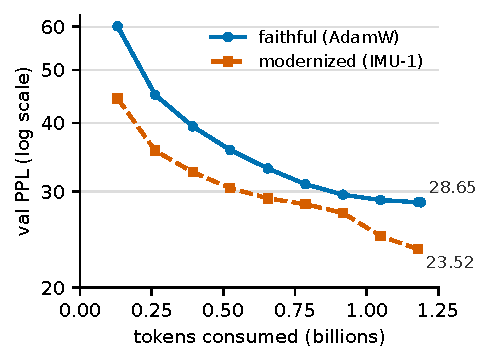
\includegraphics[width=0.72\linewidth]{figures/fig_ppl_curves.pdf}
\caption{In-loop validation perplexity versus consumed tokens for the faithful
baseline and the modernized IMU-1 build~\citep{grigorev2026imu} at the
identical 1{,}189{,}478{,}400-token budget (18{,}150 steps $\times$ 65{,}536
tok/step, FineWeb-Edu, seed 0). Single run per arm, trainer-internal
FineWeb-Edu validation eval, no suite stamp; endpoints are tabulated with
their independent suite-stamped scores in Table~\ref{tab:arms}, and no
comparative claim is drawn from these $n{=}1$ curves here. The faithful curve
ends at the post-training eval (28.65); the run completed in 2{,}663.1
minutes at 52.4\,GB peak memory. Sources:
\texttt{qwen3\_baseline2tpp\_train.log},
\texttt{qwen3\_imu1\_2tpp\_train.log}.}
\label{fig:ppl-curves}
\end{figure}

\subsection{Gap to the original}

The released \texttt{Qwen3-0.6B-Base}, trained on $\approx$36T tokens, scores
13.400 on the identical 300k-token FineWeb-Edu validation slice with identical
evaluation code (204{,}800 tokens scored, 50 windows $\times$ 4096). Our
1.19B-token baseline at 28.65 therefore sits at $2.14\times$ the original's
perplexity with $\approx$30{,}000$\times$ less data
(Figure~\ref{fig:repro-gap}). The earlier matched-compute learning-rate sweep
at $\approx$131M tokens per arm provides a second, smaller-budget point: its
best arm (peak LR $2.4\times10^{-3}$, carried forward to the full run) reached
46.310, a $3.5\times$ gap at $\approx$275{,}000$\times$ less data, with the
$1.7\times10^{-3}$ and $3.0\times10^{-3}$ arms at 46.892 and 49.276. The two
ratios belong to two different budgets and are never conflated. Both are
descriptive only -- single runs, in-loop trainer evals, no variance estimate
-- and locate the small-budget models on the same axis as the reference; they
are not parity claims.

\begin{figure}[t]
\centering
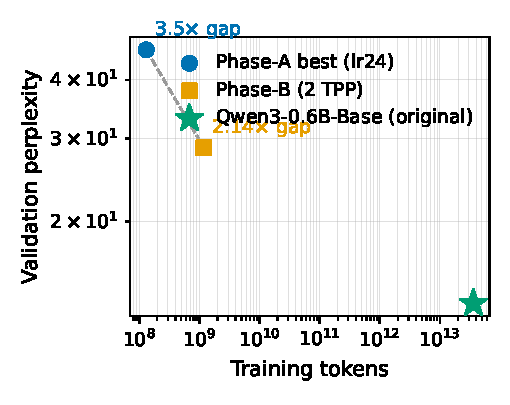
\includegraphics[width=0.72\linewidth]{figures/fig_repro_gap.pdf}
\caption{Gap to the original: validation perplexity versus training tokens on
the identical 300k-token FineWeb-Edu validation slice (204{,}800 tokens
scored, identical eval code). Original \texttt{Qwen3-0.6B-Base} 13.400 at
$\approx$36T tokens; faithful baseline 28.65 at 1{,}189{,}478{,}400 tokens
($2.14\times$ gap, $\approx$30{,}000$\times$ less data); best Phase~A
learning-rate-sweep arm 46.310 at $\approx$131M tokens ($3.5\times$ gap,
$\approx$275{,}000$\times$ less data). Single run per point, in-loop trainer
eval, not suite-stamped; descriptive only. Sources:
\texttt{original\_vs\_repro.txt}, \texttt{qwen3\_baseline2tpp\_after.txt}.}
\label{fig:repro-gap}
\end{figure}

\subsection{Suite-stamped scores for the baseline checkpoint}

Because the in-loop 28.65 lives on the trainer's own FineWeb-Edu validation
split, it is never compared against numbers from other corpora. The
independent evaluation harness stamps the same checkpoint at wikitext-2
perplexity 37.01 and code\_py perplexity 438.67 (text-lm-v2, 204{,}600 tokens
per corpus), each with a subsample noise floor -- 1.30 absolute
($\approx$3.7\%) on wikitext-2 but 280.56 absolute ($\approx$68.2\%) on
code\_py, so code-perplexity differences for this checkpoint are read as
directional only (Table~\ref{tab:arms}). These stamped values, not the
in-loop curve, are the baseline reference points for every cross-run
comparison in the following sections.
        % 5. Bit-exact reproductions + faithful 2 TPP baseline
\section{Pre-Training: From a Confounded Headline to Attributed Causes}\label{sec:pretrain}

\subsection{The motivating result: a bundle wins, but nothing is attributed}\label{sec:pretrain-motivation}

With the faithful reproduction verified (Table~\ref{tab:repro}), three builds were
trained at matched compute -- each consuming $18{,}150$ steps $\times$
$65{,}536$ tokens $= 1{,}189{,}478{,}400$ ($\approx$1.19B) FineWeb-Edu tokens
\citep{penedo2024fineweb} at sequence length 4096 on identical data, schedule
shape, and held-out validation set. The \emph{faithful} build follows the
published Qwen3 architecture \citep{yang2025qwen3}; the \emph{modernized}
build applies the IMU-1 bundle \citep{grigorev2026imu}, a package of recent
training changes; the \emph{exploratory} build applies rotary position
embeddings \citep{su2021roformer} to only a 0.25 fraction of each head's
dimensions. Table~\ref{tab:arms} reports the outcome: modernized 23.52 vs
faithful 28.65 vs partial-RoPE-0.25 29.54 in-loop validation perplexity
(single run per build, not suite-stamped); a fourth arm (partial-RoPE 0.10)
died at step $5{,}450/18{,}150$ and is excluded. The bundle's apparent margin
is $-17.9\%$ relative perplexity -- but the repository itself records that
number as $n{=}1$ and directional, and this paper treats it as motivation
rather than a result: it is a single-seed, in-loop trainer evaluation with no
variance estimate.

% tab_arms.tex -- three builds at matched 1.19B-token compute
% Sources (re-read 2026-07-06):
%   in-loop val PPLs: builds/2026-06-08_reproduce-modernized_qwen3-0.6b/results/qwen3_imu1_2tpp_train.log (line 381),
%     builds/2026-06-08_reproduce-faithful_qwen3-0.6b/results/qwen3_baseline2tpp_train.log (line 396),
%     builds/2026-06-08_reproduce-exploratory_qwen3-0.6b/results/qwen3_prope25_2tpp_train.log (line 378),
%     builds/2026-06-08_reproduce-faithful_qwen3-0.6b/results/phase_b_driver.log (RoPE-0.10 arm Terminated at step 5450)
%   text-lm-v2 suite: experiments/2026-06-16_qwen3-0.6b_eval-{modernized,faithful,prope25}/eval/suite_results.json
\begin{table}[t]
\centering
\small
\begin{tabular}{@{}lrrrrr@{}}
\toprule
 & In-loop val PPL & \multicolumn{2}{c}{wikitext-2 (text-lm-v2)} & \multicolumn{2}{c}{code\_py (text-lm-v2)} \\
\cmidrule(lr){3-4} \cmidrule(l){5-6}
Build & (FineWeb-Edu, $n{=}1$) & PPL & floor & PPL & floor \\
\midrule
Modernized (IMU-1)            & 23.52 & 27.80 & 1.07  & 129.42 & 111.92 \\
Faithful (baseline)           & 28.65 & 37.01 & 1.30  & 438.67 & 280.56 \\
Exploratory (partial-RoPE 0.25) & 29.54 & 38.08 & 1.70  & 447.30 & 298.90 \\
\bottomrule
\end{tabular}
\caption{The three Qwen3-0.6B builds at matched compute: each trained
$18{,}150$ steps $\times$ $65{,}536$ tok $= 1{,}189{,}478{,}400$
($\approx$1.19B) FineWeb-Edu tokens at sequence length 4096 (identical data,
schedule shape, and held-out val set). ``In-loop val PPL'' is the trainer's
own FineWeb-Edu validation eval -- a single run per build ($n{=}1$, no
variance estimate, no suite stamp; the IMU-1 value is the last eval, at step
18{,}000 of 18{,}150). The right four columns are the independent
\texttt{text-lm-v2} eval-harness pass on the same checkpoints (204{,}600
tokens per corpus) with its subsample noise floor (\texttt{floor\_abs});
they confirm the ordering on both corpora, but the code\_py floors are
68--92\% of the measurement (floor\_pct 92.1/68.2/70.9), so the code-PPL
gaps should be read as directional only. A fourth arm (partial-RoPE 0.10)
died at step 5{,}450/18{,}150 (last-eval PPL 50.71) and is excluded.
Sources: \texttt{qwen3\_imu1\_2tpp\_train.log},
\texttt{qwen3\_baseline2tpp\_train.log},
\texttt{qwen3\_prope25\_2tpp\_train.log}, \texttt{phase\_b\_driver.log},
and the three per-build \texttt{suite\_results.json} files.}
\label{tab:arms}
\end{table}


An independent \texttt{text-lm-v2} eval-harness pass on the same three
checkpoints (Table~\ref{tab:arms}, right columns) confirms that the
\emph{ordering} is not an artifact of the trainer's own eval: on WikiText-2
the modernized checkpoint scores 27.80 vs faithful 37.01 vs exploratory 38.08
(a 24.9\% relative gap between modernized and faithful), and the Python-code
corpus preserves the same ranking, though its subsample noise floors are
68--92\% of the measurement, so the code gaps are directional only.
Figure~\ref{fig:ppl-curves} shows the two in-loop validation curves at the
identical 1.19B budget.

The problem is that IMU-1 is a \emph{bundle}: it changes roughly six things at
once -- the NorMuon optimizer \citep{li2025normuon}, a warmup-stable-decay
(WSD) learning-rate schedule \citep{hu2024minicpm}, a z-loss regularizer
\citep{chowdhery2022palm}, and a three-flag architecture package
(value-residual connections, layernorm scaling, and attention head gating)
\citep{grigorev2026imu}. A single $n{=}1$ perplexity delta cannot say which of
these mattered. The remainder of this section attributes the gain through
single-variable, iso-FLOP, multi-seed ablations: first the optimizer in
isolation, then a factored de-confound of the remaining axes.

\subsection{Optimizer isolation: NorMuon vs AdamW}\label{sec:pretrain-optimizer}

The optimizer axis was isolated in a single-variable A/B: NorMuon
\citep{li2025normuon} vs AdamW \citep{loshchilov2017decoupled} on the 196 2D
hidden weight matrices, with embeddings and all 1D parameters remaining under
AdamW in \emph{both} arms, so the arms differ only in the update rule applied
to the hidden matrices. Each cell trains a fixed $640$ steps $\times$
$65{,}536$ tokens $= 41{,}943{,}040$ ($\approx$42M) tokens -- iso-FLOP by
construction -- with 3 seeds per arm, paired. Table~\ref{tab:attrib} (top row)
gives the result under \texttt{text-lm-v2}: NorMuon improves bits-per-byte by
$+0.4743$ on WikiText-2 (95\% CI $[+0.4435, +0.5052]$, 3 seeds, paired) and
$+0.5016$ on code (95\% CI $[+0.4560, +0.5471]$, 3 seeds, paired), both
significant. Two hedges bound this claim. First, it is scoped as an
early-training optimization-speed signal at one architecture and one small
budget; it is \emph{not} a claim that the advantage persists at scale or to
convergence. Second, seeds vary initialization and data-shuffle order on a
fixed data split, so the CIs may understate fully randomized run-to-run
variance.

% tab_attrib.tex -- attribution: single-variable iso-FLOP ablations
% Sources (re-read 2026-07-06):
%   experiments/2026-06-16_qwen3_normuon-vs-adamw/results/verdict.json (+ results/lr_sweep_bpb.json, RESULT.md)
%   experiments/2026-06-18_qwen3-0.6b_imu1-deconfound-p1/verdict.json (+ c5_evidence.json)
%   experiments/2026-06-21_qwen3-0.6b_arch-subdrill-p2/verdict.json (+ c5_evidence.json)
\begin{table}[t]
\centering
\small
\setlength{\tabcolsep}{3pt}
\begin{tabular}{@{}llrlcrlc@{}}
\toprule
 & & \multicolumn{3}{c}{wikitext-2} & \multicolumn{3}{c}{code\_py} \\
\cmidrule(lr){3-5} \cmidrule(l){6-8}
Study & Axis & $\Delta$BPB & 95\% CI & sig. & $\Delta$BPB & 95\% CI & sig. \\
\midrule
Optimizer (42M tok) & NorMuon vs AdamW & $+0.4743$ & $[+0.4435, +0.5052]$ & yes & $+0.5016$ & $[+0.4560, +0.5471]$ & yes \\
\midrule
Phase 1 (131M tok)  & wsd   & $+0.0245$ & $[-0.0173, +0.0662]$ & n.s. & $+0.0361$ & $[-0.0649, +0.1372]$ & n.s. \\
                    & zloss & $-0.0034$ & $[-0.0175, +0.0108]$ & n.s. & $-0.0007$ & $[-0.0522, +0.0508]$ & n.s. \\
                    & arch  & $+0.1179$ & $[+0.1005, +0.1354]$ & yes  & $+0.3049$ & $[+0.2588, +0.3511]$ & yes \\
\midrule
Phase 2 (131M tok)  & vr    & $+0.0355$ & $[+0.0116, +0.0594]$ & yes  & $+0.1072$ & $[+0.0492, +0.1651]$ & yes \\
                    & ln    & $+0.0337$ & $[+0.0175, +0.0498]$ & yes  & $+0.0606$ & $[+0.0198, +0.1013]$ & yes \\
                    & hg    & $+0.0256$ & $[+0.0125, +0.0386]$ & yes  & $+0.0422$ & $[+0.0081, +0.0763]$ & yes \\
\bottomrule
\end{tabular}
\caption{Attribution of the IMU-1 bundle via single-variable iso-FLOP
ablations ($\Delta$BPB $>0$ means the treatment improves bits-per-byte over
the faithful AdamW baseline; all numbers \texttt{text-lm-v2}-stamped,
$n{=}3$ seeds per arm with 95\% Welch-$t$ CIs). Optimizer row: NorMuon vs
AdamW on the 196 2D hidden weights only (embeddings/1D AdamW in both arms)
at a fixed 41{,}943{,}040-token ($\approx$42M) budget per cell, 640 steps
$\times$ 65{,}536 tok, iso-FLOP by construction; a matched-config AdamW LR
sweep (1.7/3.5/4.8e-3 single-seed plus the 3-seed 2.4e-3 anchor) spans only
$\sim$0.047 BPB, $\sim$10x smaller than the gap, so no swept AdamW LR closes
it; scoped as an early-training optimization-speed signal, not a scale
claim. Phase 1/Phase 2 rows: 2000 steps $\times$ 65{,}536 tok
$= 131{,}072{,}000$ tokens per cell against a shared 3-seed baseline
(Phase 2 reuses the Phase-1 baseline checkpoints, re-scored in-cohort);
iso-FLOP confirmed within the 5\% gate (largest deviation: arch/hg
$+0.077\%$ params, FLOP ratio 1.00043). Phase 1 finds \emph{arch} the only
significant driver (drivers $=$ [arch], verdict ``attributed''); Phase 2
splits arch into value-residual (vr), layernorm-scaling (ln), and
head-gating (hg), each individually significant on both corpora (drivers
$=$ [vr, ln, hg]). Sources: \texttt{verdict.json} of the three experiments
plus \texttt{lr\_sweep\_bpb.json}.}
\label{tab:attrib}
\end{table}


A natural objection is an undertuned baseline. A matched-config AdamW
learning-rate sweep across $1.7\mathrm{e}{-3}$--$4.8\mathrm{e}{-3}$
(Table~\ref{tab:attrib} caption) spans only $\approx$0.047 BPB end to end --
roughly $10\times$ smaller than the $+0.474$ gap -- so no swept AdamW learning
rate comes close to closing it; the result is ``NorMuon vs AdamW anywhere in a
reasonable LR range,'' not ``NorMuon vs one AdamW point.'' Caveats: the three
off-anchor sweep points are single-seed (only the $2.4\mathrm{e}{-3}$ anchor
has 3 seeds), and weight decay was held at $0.1$ for both arms rather than
retuned per optimizer. The speed signal is also not free: NorMuon ran at
$\approx$6{,}664 tokens/s vs AdamW's $\approx$7{,}340 tokens/s in these cells,
a $\approx$9\% wall-clock throughput overhead.

\subsection{De-confound Phase 1: which axis of the bundle drives the gain?}\label{sec:pretrain-p1}

Phase 1 factors the non-optimizer axes of the bundle -- \emph{wsd} (schedule),
\emph{zloss} (regularizer), and \emph{arch} (the three architecture flags as
one unit) -- each ablated single-variable against the faithful AdamW baseline
at $2000$ steps $\times$ $65{,}536$ tokens $= 131{,}072{,}000$ tokens per
cell, 3 seeds per arm (12 cells total). The baseline arm was re-verified
bit-exact against the canonical model (max $|\Delta \text{logits}| = 0.0$)
before launch, and the comparison is iso-FLOP: the arch arm adds only
$+0.077\%$ parameters, a FLOP ratio of 1.00042, well inside the 5\% gate.

Figure~\ref{fig:deconfound} (panel A) and Table~\ref{tab:attrib} show the
outcome: \emph{only the architecture axis is significant}, with $+0.1179$ BPB
on WikiText-2 (95\% CI $[+0.1005, +0.1354]$, 3 seeds, paired) and $+0.3049$ on
code (95\% CI $[+0.2588, +0.3511]$, 3 seeds, paired). The schedule and z-loss
axes are not significant on either corpus -- their CIs straddle zero
(Table~\ref{tab:attrib}). The recorded verdict is ``attributed'' with drivers
$=$ [arch]: at this budget, neither the WSD schedule nor the z-loss
regularizer contributes a measurable quality gain.

\begin{figure}[t]
\centering
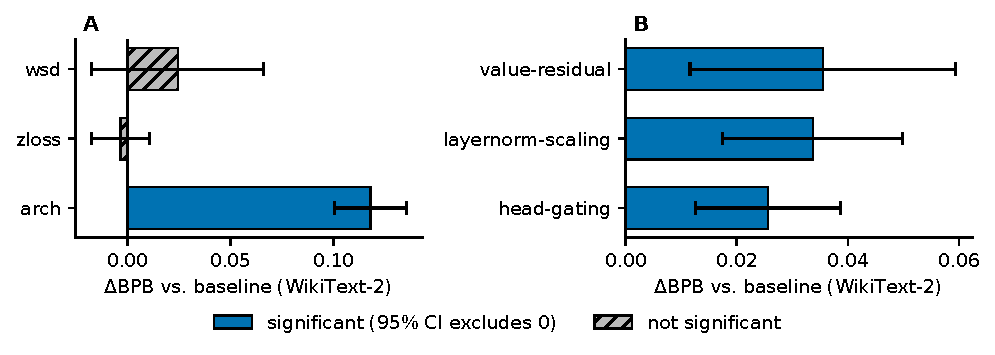
\includegraphics[width=\linewidth]{figures/fig_deconfound.pdf}
\caption{De-confounding the IMU-1 bundle on WikiText-2 BPB improvement over
the faithful AdamW baseline (positive $=$ better). Panel A: Phase-1 axes --
wsd (schedule), zloss (regularizer), arch (the three-flag architecture
bundle). Panel B: Phase-2 sub-drill of the arch bundle into value-residual,
layernorm-scaling, and head-gating, scored against the reused Phase-1
baseline checkpoints. Every cell trains $2000$ steps $\times$ $65{,}536$
tokens $= 131{,}072{,}000$ tokens; $n{=}3$ seeds per arm; error bars are
95\% CIs; hatched grey bars are not significant. Iso-FLOP holds within the
5\% gate for all arms (largest deviation $+0.077\%$ parameters, FLOP ratio
1.00043); all numbers are \texttt{text-lm-v2}-stamped. Sources:
\texttt{verdict.json} of experiments
\texttt{2026-06-18\_qwen3-0.6b\_imu1-deconfound-p1} and
\texttt{2026-06-21\_qwen3-0.6b\_arch-subdrill-p2}, plotted by
\texttt{fig\_deconfound.py}.}
\label{fig:deconfound}
\end{figure}

\subsection{De-confound Phase 2: splitting the architecture bundle}\label{sec:pretrain-p2}

Phase 2 drills into the winning arch axis, ablating its three flags
individually -- value-residual (vr), layernorm-scaling (ln), and head-gating
(hg) -- at the same $131{,}072{,}000$ tokens per cell and 3 seeds per arm
(9 new cells). Rather than re-training a baseline, Phase 2 reuses the
Phase-1 baseline checkpoints (identical optimizer, schedule, budget, seeds,
and data) and re-scores them in-cohort, so every comparison shares one
control. Iso-FLOP again holds by a wide margin: value-residual adds 84
parameters, layernorm-scaling adds none, and head-gating adds $458{,}752$
($+0.077\%$, FLOP ratio 1.00043).

Each flag is individually significant on both corpora
(Figure~\ref{fig:deconfound}, panel B; Table~\ref{tab:attrib}): on WikiText-2,
value-residual $+0.0355$ BPB (95\% CI $[+0.0116, +0.0594]$),
layernorm-scaling $+0.0337$ (95\% CI $[+0.0175, +0.0498]$), and head-gating
$+0.0256$ (95\% CI $[+0.0125, +0.0386]$), all at 3 seeds, paired; the code
corpus shows the same pattern at larger magnitudes (Table~\ref{tab:attrib}).
The three single-flag WikiText-2 effects are near-additive: their sum,
$\approx$0.0947 BPB, approaches the bundled arch effect of $+0.1179$ BPB from
Phase 1, leaving only a small residual for interactions and seed noise. The
Phase-2 verdict is again ``attributed,'' with drivers $=$ [vr, ln, hg].

\subsection{What the headline actually was}\label{sec:pretrain-summary}

The attribution chain replaces one unexplained $-17.9\%$ ($n{=}1$, in-loop)
headline with four small, separately measured causes: an optimizer
optimization-speed effect ($+0.47$ BPB at a 42M-token budget, scoped to early
training) and three individually significant architecture effects
(value-residual, layernorm-scaling, head-gating; together $\approx$0.09 of
the $+0.12$ BPB bundled arch gain at 131M tokens) -- while the schedule and
z-loss axes, plausible-sounding members of the same bundle, contributed
nothing measurable at these budgets. None of these attributed effects is a
scale claim; all are 3-seed, iso-FLOP, \texttt{text-lm-v2}-stamped
comparisons at 42M--131M-token proxy budgets on a 596M-parameter model.
         % 6. Pre-training attribution (optimizer, de-confound p1/p2)
\section{Data Composition}\label{sec:data}

Data composition is among the highest-leverage levers reported for small-model pretraining \citep{penedo2024fineweb, li2024datacomp, allal2025smollm2}, and it is also the axis most cheaply isolated: holding the model, optimizer, schedule, and token budget fixed while swapping only the training corpus yields an iso-FLOP comparison by construction. This section tests two treatments against the FineWeb-Edu \citep{penedo2024fineweb} distribution used for the faithful base: (i) dclm-edu, a curated corpus derived from DCLM \citep{li2024datacomp}, and (ii) a 50/50 dclm-edu\,+\,FineWeb-Edu mix. Every cell trains the identical 596M model for 2{,}000 steps $\times$ 65{,}536 tokens $=$ 131{,}072{,}000 ($\approx$131M) tokens with 3 seeds per arm; only the data differs, so the train-FLOP ratio across arms is 1.000. Following the control-reuse protocol, the FineWeb-Edu control checkpoints are the reused Phase-1 de-confound baselines (symlinked and re-scored in-cohort), and the mix experiment likewise reuses the dclm-edu arm rather than retraining it. The dclm-edu shards were decontaminated against both evaluation corpora (13-gram overlap; zero documents dropped). All effects below are bits-per-byte (BPB) improvements over the control with paired across-seed 95\% CIs (text-lm-v2); Table~\ref{tab:data} gives the full cell values.

% tab_data.tex -- data-composition head-to-head: dclm-edu and 50/50 mix vs FineWeb-Edu control.
% Sources: verdict.json + cohort_bpb.json in
%   Qwen3-0.6B/experiments/2026-06-24_qwen3-0.6b_data-dclm-vs-fineweb/ (dclm arm)
%   Qwen3-0.6B/experiments/2026-06-26_qwen3-0.6b_data-mix-composition/ (mix arm; reuses the dclm arm and the FineWeb controls)
\begin{table}[t]
\centering
\caption{Pretraining data composition at 596M: \textbf{dclm-edu} and a \textbf{50/50 dclm-edu\,+\,FineWeb-Edu mix} vs.\ a FineWeb-Edu control.
Every cell trains the identical model for 2{,}000 steps $\times$ 65{,}536 tokens $=$ 131{,}072{,}000 ($\approx$131M) tokens ($n{=}3$ seeds per arm); only the data differs, so the arms are iso-FLOP by construction (train-FLOP ratio 1.000).
$\Delta$BPB $=$ control BPB $-$ arm BPB (positive $=$ arm better); 95\% CIs are paired across-seed; ``sig.''\ means the CI excludes zero.
FineWeb-Edu control checkpoints are reused baselines (control-reuse policy); the mix experiment reuses the dclm arm.
On code, the mix retains $0.5904/0.7034 = 83.9\%$ of the pure-dclm improvement while directionally \emph{improving} English (dclm alone directionally hurts it, n.s.).
Eval suite: \texttt{text-lm-v2} (BPB with the model's own tokenizer; wikitext-2 val 869{,}710 bytes, Python code 843{,}643 bytes, 204{,}600 tokens per corpus per cell).
Source files: \texttt{verdict.json}, \texttt{cohort\_bpb.json}, \texttt{c5\_evidence.json}, \texttt{run\_arms.sh} (experiments 2026-06-24 dclm-vs-fineweb and 2026-06-26 data-mix-composition).}
\label{tab:data}
\footnotesize
\begin{tabular}{llccccc}
\toprule
Arm & Corpus & Control BPB & Arm BPB & $\Delta$BPB & 95\% CI & sig.\ \\
\midrule
dclm-edu      & code (Python)  & 2.6385 & 1.9351 & $+0.7034$ & $[+0.6639,\,+0.7430]$ & yes \\
dclm-edu      & wikitext-2     & 1.5157 & 1.5254 & $-0.0097$ & $[-0.0255,\,+0.0061]$ & no  \\
\addlinespace
50/50 mix     & code (Python)  & 2.6385 & 2.0481 & $+0.5904$ & $[+0.5532,\,+0.6277]$ & yes \\
50/50 mix     & wikitext-2     & 1.5157 & 1.4996 & $+0.0161$ & $[-0.0005,\,+0.0327]$ & no  \\
\bottomrule
\end{tabular}
\end{table}


\paragraph{dclm-edu vs.\ FineWeb-Edu.} On the Python-code corpus, dclm-edu improves BPB by $+0.7034$ (95\% CI $[+0.6639, +0.7430]$, 3 seeds, paired), significant, and by far the largest single effect measured in this study (Table~\ref{tab:data}). The underlying perplexities make the scale concrete: per-seed code perplexity falls from $\approx$1{,}890 under the FineWeb-Edu control (seed range 1{,}804--1{,}962) to $\approx$250 under dclm-edu (seed range 245--266) --- the control corpus simply contains too little code-like text for the model to acquire the distribution. On wikitext-2, dclm-edu is directionally worse, $-0.0097$ BPB (95\% CI $[-0.0255, +0.0061]$, 3 seeds, paired), not significant (text-lm-v2). Pure dclm-edu therefore buys a large code gain at a possible, unresolved English cost.

\paragraph{The 50/50 sequence-preserving mix.} The mix arm concatenates equal token counts from the two sources as coherent halves; packing then produces 4{,}096-token windows each drawn from a single source, and the loader shuffles at the packed-sequence level, so document structure survives mixing. At the same matched 131M-token budget, the mix improves code BPB by $+0.5904$ (95\% CI $[+0.5532, +0.6277]$, 3 seeds, paired), significant --- $0.5904/0.7034 = 83.9\%$ of the pure-dclm code improvement, a well-defined ratio because both effects are measured against the same FineWeb-Edu baseline (Table~\ref{tab:data}). On wikitext-2 the mix shows $+0.0161$ BPB (95\% CI $[-0.0005, +0.0327]$, 3 seeds, paired), not significant but with a positive point estimate: English is preserved rather than traded away (text-lm-v2). The mix is thus best-of-both at this scale --- it keeps the English performance the pure treatment put at risk while retaining most of the code win --- and it becomes the anneal ingredient for mid-training (Figure~\ref{fig:data-anneal}).

\paragraph{An invalid first run, caught by implausibility.} The first mix cohort was invalid: the data loader interleaved the two sources with a token-level shuffle, which destroyed all sequence structure and produced token soup. The evidence gate flagged the failure before any code inspection --- the broken mix scored roughly twice the BPB of \emph{both} pure arms on both corpora, which is physically implausible for a blend of two individually healthy distributions. The cohort was discarded, the mixing was rewritten to be sequence-preserving (fix commit \texttt{a576baa}), and the arm was retrained from scratch. Section~\ref{sec:failures} gives the full account, including the diagnostic probe that confirmed the repair.

\paragraph{Bookkeeping.} The ledger records both runs with verdict \emph{directional}, a conservative cap; the per-corpus significance keys in each \texttt{verdict.json} are the authoritative numbers, and the mix verdict file's overall-verdict string is a recipe-level template that should not be read against them. One protocol deviation is noted rather than papered over: the mix experiment carries no \texttt{c5\_evidence.json} of its own --- its budget and single-variable confound evidence live in \texttt{run\_arms.sh} together with the reused dclm-experiment \texttt{c5\_evidence.json}.
                % 7. Data composition (dclm-edu, 50/50 mix)
\section{Mid-Training: Premium-Data Annealing and the Context Gate}\label{sec:midtrain}

Mid-training -- the interval between the main pretraining run and post-training -- offered two candidate interventions for the 596M base: extending the context window, and annealing onto premium data during a learning-rate cooldown \citep{hu2024minicpm, olmo20242}. The first was killed by a cheap diagnostic before any budget was spent; the second is the one stage in this study that reaches a \emph{win} under the per-stage eval-completeness gate. Table~\ref{tab:midtrain} summarizes the stage.

% tab_midtrain.tex -- mid-training anneal (premium mix) vs iso-token FineWeb control vs un-annealed base.
% Sources: verdict.json (corpora, short_ctx_non_regression, ecl_ladder), c5_evidence.json in
%   Qwen3-0.6B/experiments/2026-06-30_qwen3-0.6b_midtrain-anneal/
%   step0 gate: Qwen3-0.6B/experiments/2026-06-27_qwen3-0.6b_midtraining/step0_diagnostic.json
\begin{table}[t]
\centering
\caption{Mid-training anneal at 596M: premium-mix anneal vs.\ an iso-token FineWeb-Edu control vs.\ the un-annealed base.
Both arms run the identical 1-sqrt cooldown (peak LR $2.5\times10^{-4} \rightarrow 2.5\times10^{-5}$, 10\% floor) for 2{,}300 steps $\times$ 65{,}536 tokens $=$ 150.7M tokens per cell ($\approx$13\% of the 1.19B-token pretrain), $n{=}3$ seeds per arm; only the data differs (iso-FLOP by construction).
Top block: BPB per corpus, with the anneal$-$control improvement and its paired across-seed 95\% CI (suite \texttt{text-lm-v2}).
The control barely moves off the base ($+0.0050$ code, $+0.0036$ wikitext-2 BPB), i.e.\ LR decay plus 150M extra FineWeb tokens alone do approximately nothing --- the data, not the schedule, carries the effect.
The wikitext-2 gain is small but significant, violating the pre-registered expected null on English; it is reported as-is.
Bottom block: effective-context-length passkey ladder (suite \texttt{ecl-ladder-v1}, $n{=}40$ probes per rung per cell, arms pooled over 3 seeds, Wilson 95\% CIs); the base's anomalous 4096-rung accuracy (exactly 0.025) is repaired to 0.400 by both arms, and no cell regresses vs.\ base at any rung.
A separate step-0 diagnostic (\texttt{step0\_diagnostic.json}) had gated context \emph{extension} to propose-only: the base scores 0.083 at its own 4096-token trained window (threshold 0.5, gate FAIL).
Source files: \texttt{verdict.json}, \texttt{c5\_evidence.json} (2026-06-30 midtrain-anneal), \texttt{step0\_diagnostic.json} (2026-06-27 midtraining).}
\label{tab:midtrain}
\footnotesize
\setlength{\tabcolsep}{3.5pt}
\begin{tabular}{lcccc}
\toprule
 & Base & Control (FineWeb) & Anneal (mix) & Anneal $-$ Control (95\% CI) \\
\midrule
\multicolumn{5}{l}{\emph{BPB (lower is better; improvements are positive), suite \texttt{text-lm-v2}}} \\
Code (Python) BPB        & 2.1286 & 2.1236 & 1.8520 & $+0.2716$ $[+0.2641,\,+0.2792]$ sig.\ \\
wikitext-2 BPB           & 1.2256 & 1.2220 & 1.2062 & $+0.0157$ $[+0.0140,\,+0.0174]$ sig.\ \\
$\Delta$ vs.\ base, code       & --- & $+0.0050$ & $+0.2766$ & \\
$\Delta$ vs.\ base, wikitext-2 & --- & $+0.0036$ & $+0.0194$ & \\
\midrule
\multicolumn{5}{l}{\emph{Passkey accuracy by context rung (suite \texttt{ecl-ladder-v1}; Wilson 95\% CI; arms pooled, $3{\times}40$ probes)}} \\
512-token rung  & 0.200 $[0.105,\,0.348]$ & 0.308 $[0.233,\,0.396]$ & 0.817 $[0.738,\,0.876]$ & \\
4096-token rung & 0.025 $[0.004,\,0.129]$ & 0.400 $[0.317,\,0.489]$ & 0.400 $[0.317,\,0.489]$ & \\
\bottomrule
\end{tabular}
\end{table}


\subsection{The step-0 diagnostic that gated off context extension}\label{sec:midtrain-gate}

Before budgeting a context-extension run, a step-0 passkey-retrieval diagnostic \citep{mohtashami2023landmark} probed the base checkpoint at and beyond its trained window. The pre-registered gate required accuracy $\geq 0.5$ at the trained length of 4096 tokens; the base scored 0.083 (Table~\ref{tab:midtrain}). Per-length accuracies were 0.333 at 512, 1024, and 2048 tokens, 0.083 at 4096, 0.583 at 6144, and 0.250 at 8192. The diagnostic nominally reports an effective context length of 6144 because the 6144-token rung happens to clear the absolute threshold, but the ladder is non-monotone and the above-trained-window spike at 6144 is better read as instability of a small unstamped probe than as genuine capability; the decision variable is the trained-length accuracy, and it failed by a factor of six. The recorded verdict is that context extension is moot -- the base collapses \emph{before} its trained window -- so the extension sub-stage stayed propose-only and no extension run was launched. This is the pattern that effective-context benchmarks document at much larger scales, where usable context falls well short of the nominal window \citep{hsieh2024ruler}; here the gap is severe enough at 596M and 1.19B training tokens that extending the nominal window would optimize the wrong margin.

\subsection{Annealing onto the premium mix under an iso-token control}\label{sec:midtrain-anneal}

The anneal starts from the faithful base checkpoint (1.19B FineWeb-Edu tokens \citep{penedo2024fineweb}) and runs a ``1-sqrt'' cooldown from peak learning rate $2.5\times10^{-4}$ to $2.5\times10^{-5}$ (a 10\% floor, 46 warmup steps) for 2{,}300 steps $\times$ 65{,}536 tokens $=$ 150.7M tokens per cell, $\approx$13\% of the pretraining budget, with $n{=}3$ seeds per arm. The treatment anneals onto the 50/50 dclm-edu/FineWeb-Edu mix selected by the data-composition study \citep{li2024datacomp} (Table~\ref{tab:data}); the control runs the identical cooldown on iso-token FineWeb-Edu. Exactly one variable (the data) differs, so the comparison is iso-FLOP by construction, and the design eats the standard confound of anneal experiments: whatever the learning-rate decay plus 150M additional tokens do on their own is captured by the control.

The answer is that they do approximately nothing. The control moved $+0.0050$ BPB on code and $+0.0036$ BPB on wikitext-2 relative to the un-annealed base (text-lm-v2; Table~\ref{tab:midtrain}), while the mix anneal beat the control on code by $+0.2716$ BPB (95\% CI $[+0.2641, +0.2792]$, 3 seeds, paired), significant (text-lm-v2; Figure~\ref{fig:data-anneal}). The data, not the schedule, carries the effect. Against the constant-learning-rate continued-train sibling on the same mix ($+0.5904$ BPB on code, 95\% CI $[+0.5532, +0.6277]$; an upper-bound reference at a similar 131M-token budget, not an iso-FLOP comparison), the 150.7M-token cooldown retains $\approx$46\% of the effect.

On English, the pre-registration expected an honest null; the measurement violated it: wikitext-2 improved by $+0.0157$ BPB (95\% CI $[+0.0140, +0.0174]$, 3 seeds, paired), significant (text-lm-v2), $\approx$1.3\% relative. This is reported as an exploratory violation of the pre-registered expectation, not as a claim: the point estimate is the same size as the constant-learning-rate sibling's $+0.0161$ BPB, which was \emph{not} significant, and what pushed the anneal's identical-size effect past significance is the cooldown's much tighter across-seed spread. A same-size estimate flipping significance purely through variance is exactly the situation pre-registration exists to flag.

\begin{figure}[t]
\centering
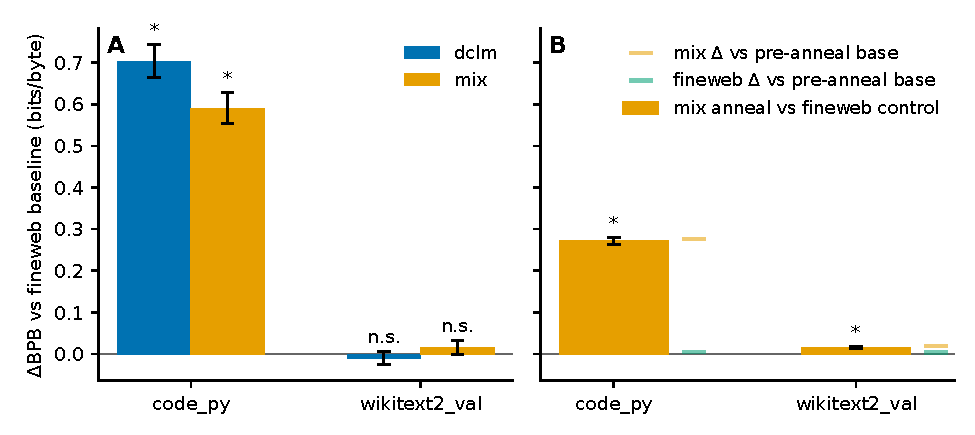
\includegraphics[width=\linewidth]{figures/fig_data_anneal}
\caption{Data-composition and mid-training-anneal effects: BPB improvement over the FineWeb-Edu control (positive is better) with paired across-seed 95\% CIs, $n{=}3$ seeds per arm, suite \texttt{text-lm-v2}, on \texttt{code\_py} and wikitext-2. Data-composition arms (dclm-edu; 50/50 mix) train 2{,}000 steps $\times$ 65{,}536 $=$ 131.1M tokens per cell at full LR; the mid-training anneal arms run the 1-sqrt cooldown for 2{,}300 steps $\times$ 65{,}536 $=$ 150.7M tokens per cell ($\approx$13\% of the 1.19B-token pretrain) against an iso-token FineWeb-Edu control. Sources: \texttt{verdict.json} of the 2026-06-24 dclm-vs-fineweb, 2026-06-26 data-mix-composition, and 2026-06-30 midtrain-anneal experiments; rendered by \texttt{fig\_data\_anneal.py}.}
\label{fig:data-anneal}
\end{figure}

\subsection{The effective-context-length ladder}\label{sec:midtrain-ecl}

Both anneal arms and the base were then scored on a passkey ladder over context rungs 512--8192 (ecl-ladder-v1; $n{=}40$ probes per rung per cell, arms pooled over 3 seeds, Wilson 95\% CIs; Figure~\ref{fig:ecl-ladder}). The base exhibits an anomalous dip at its own trained length: 4096-rung accuracy is exactly 0.025, far below its 512-rung 0.200. Both anneal arms repair the dip to 0.400 -- the FineWeb-Edu control included, so the repair does not require the premium data. The mix arm additionally lifts the pooled 512-token rung to 0.8167 versus 0.20 for the base, and no cell regresses relative to the base at any rung (the recorded regression list is empty). The mechanism of the trained-length dip, and of its repair by an ordinary cooldown, is unexplained; with $n{=}40$ probes per rung the ladder characterizes the phenomenon without diagnosing it, and it is flagged as an open question in Section~\ref{sec:limitations}. The step-0 diagnostic's independent 4096-token failure (0.083) is consistent with the same anomaly.

\begin{figure}[t]
\centering
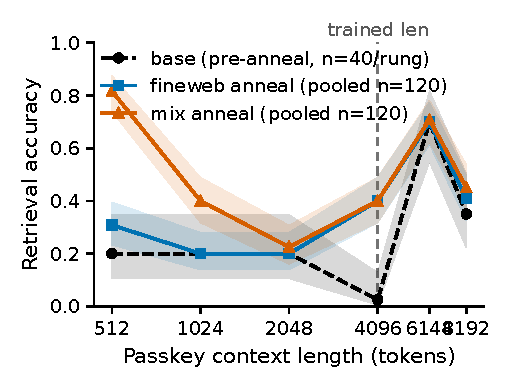
\includegraphics[width=\linewidth]{figures/fig_ecl_ladder}
\caption{Effective-context-length passkey ladder (suite \texttt{ecl-ladder-v1}): accuracy by context rung (512--8192 tokens) for the un-annealed base, the FineWeb-Edu-anneal control, and the mix-anneal treatment. $n{=}40$ probes per rung per cell; anneal arms pooled over 3 seeds ($3\times40$ probes per point); Wilson 95\% CIs. Both anneal arms (150.7M tokens per cell, identical cooldown) repair the base's anomalous 4096-rung dip ($0.025 \rightarrow 0.400$), and no cell regresses versus the base at any rung. Sources: \texttt{ecl\_ladder.json} and \texttt{verdict.json} (2026-06-30 midtrain-anneal); rendered by \texttt{fig\_ecl\_ladder.py}.}
\label{fig:ecl-ladder}
\end{figure}

\subsection{Robustness and the stage verdict}\label{sec:midtrain-verdict}

Two integrity checks qualify the headline. First, one treatment cell (mix, seed 0) was twice terminated by an external SIGTERM (exit code 143; not the resource watchdog, whose kill line was never approached) and resumed; the resume rebuilds the data shuffle without fast-forwarding, which if anything disadvantages the treatment. Excluding that cell entirely, the code effect holds: $+0.2717$ BPB (95\% CI $[+0.2333, +0.3100]$), significant, with the caveat that the treatment arm drops to $n{=}2$ seeds and the CI widens accordingly; the excluded cell's BPB (1.8521) is not a within-arm outlier (arm range 1.8489--1.8550). Second, the loaded token pools differ by $\approx$0.7\% in the control's favor, and the control lost anyway -- the imbalance is conservative with respect to the conclusion.

Under the per-stage eval-completeness gate, mid-training required three hard items -- the effective-context-length ladder, short-context non-regression, and the anneal gain against an iso-token control -- and all three are present, with the single-variable iso-FLOP check recorded in the run ledger. Mid-training is therefore the one lifecycle stage in this study that is hard-complete under the gate, and its recorded verdict is \emph{win}.
         % 8. Mid-training anneal + ECL ladder + context gate
\section{Supervised Fine-Tuning: The Win That Was Not}\label{sec:sft}

The supervised fine-tuning (SFT) stage poses a single-variable question: does
response masking --- computing the loss only on response tokens, the standard
practice in instruction tuning --- improve a small reasoning-SFT recipe over
plain continued pre-training on the same data? The stage produced the study's
most instructive de-confound: an apparently significant 0.68-PPL win for
masking that turned out to be an artifact of scoring the two arms on different
token sets, and that collapsed to roughly a hundredth of a perplexity point
under a corrected protocol (Figure~\ref{fig:sft-confound},
Table~\ref{tab:sft}).

\paragraph{Setup.}
Both arms start from the faithful 1.19B-token base checkpoint and take one
pass over the same prepared OpenR1-Math reasoning corpus of 125{,}000{,}592
tokens, in the spirit of small-model reasoning distillation
\citep{xu2026vibethinker}: peak learning rate $5\times10^{-5}$ with cosine
decay to $8\times10^{-8}$, 5\% warmup, global batch 128 (micro-batch 4, 32
accumulation steps), AdamW \citep{loshchilov2017decoupled}, $n{=}3$ seeds per
arm (Table~\ref{tab:hparams}). The treatment applies a response mask; the
control is an iso-FLOP \texttt{--no\_mask} continued-pretrain arm that is
identical in data, ordering, schedule, steps, and token budget --- the loss
mask is the only variable. Because prompts are a small fraction of this
corpus, the masked arm takes loss on 97.6\% of tokens versus the control's
100\%; the treatment effect being tested is therefore the exclusion of a thin
prompt-token slice from the objective.

\paragraph{The advisory in-loop result.}
The in-loop evaluation (training-loop perplexity, not suite-stamped, $n{=}3$
seeds per arm) showed SFT at 11.595 versus the control at 12.273 --- a
$+0.679$ gap with a tight interval (95\% CI $[+0.676, +0.681]$) that would
read as a decisive win (Table~\ref{tab:sft}, top block). But the comparison is
confounded: each arm reused its own training mask at evaluation time, so the
SFT arm was scored on response tokens only while the control was scored on all
tokens. Perplexities over different token sets are not comparable numbers. The
in-loop verdict flagged this itself and capped the result to directional,
advisory-only, pending re-scoring under a shared protocol.

\paragraph{The corrected protocol.}
The verdict of record re-scores all seven checkpoints (base plus three seeds
per arm) on one fixed held-out response-masked reasoning set: 66 held-out
OpenR1-Math documents comprising 228{,}529 response tokens, produced by a
seeded document-level split with 13-gram deduplication against the training
set. On this common footing, base perplexity 14.127 falls to 11.573 (SFT) and
11.582 (control) --- improvements of 18.1\% and 18.0\% respectively --- and
the 0.68-PPL gap collapses to $+0.009$ PPL (95\% CI $[+0.0045, +0.0139]$,
$n{=}3$ seeds per arm), nominally significant but a small fraction of the
advisory number. A tokenizer-free full-sequence cross-check
on the same documents flips the sign: $-0.006$ PPL (95\% CI $[-0.011,
-0.001]$) with the control ahead, scored not significant under the
pre-specified one-sided improvement test. Since the masked and full-sequence
comparisons disagree, the recorded verdict is \emph{directional}: the two arms
are not yet separable. Across-seed spread on the held-out set is 0.001 PPL
within the SFT arm and 0.004 PPL within the control arm, so the ambiguity is
not seed noise --- the effect itself sits at the scale of the measurement.

\paragraph{Forgetting probe.}
Neither arm damages the base distribution. On a held-out FineWeb-Edu probe
\citep{penedo2024fineweb}, base perplexity 21.495 rises to 21.652 (SFT) and
21.660 (control), a $+0.7\%$ shift (Table~\ref{tab:sft}, bottom block). On the
standard suite (text-lm-v2, one representative seed per arm), wikitext-2 moves
from 37.010 to 37.082/37.084 against a noise floor of 1.304, and the code
corpus from 438.673 to 425.689/425.594 against a floor of 280.564 --- both
labeled retained/not significant. The three-seed confidence intervals in this
section apply to the in-domain reasoning set only; the standard-suite
retention numbers are single-seed spot checks.

\paragraph{Interpretation.}
The real effect at this scale is the \emph{data}, not the masking: continued
training on in-domain mathematical reasoning delivers essentially the entire
18\% perplexity gain, and excluding the 2.4\% prompt-token slice from the loss
adds at most a hundredth of a perplexity point of separation, of ambiguous
sign. The headline that response-masked SFT beats continued pre-training does
not survive an honest iso-FLOP control. The methodological point generalizes:
a comparison whose arms are scored on different token sets can manufacture an
apparent effect nearly two orders of magnitude larger than the corrected
estimate, while presenting a confidence interval tight enough to look
unimpeachable. The study's evidence gates treated the in-loop number as
advisory by construction; the fixed held-out set, defined once and shared
across all arms, is what the verdict rests on.

% tab_sft.tex -- SFT (response-masked) vs iso-FLOP --no_mask control vs base, with the confounded
% in-loop advisory numbers shown next to the corrected held-out re-score.
% Sources in Qwen3-0.6B/experiments/2026-06-27_qwen3-0.6b_sft-3seed/:
%   verdict.json (in-loop advisory, CONFOUND key), reasoning_verdict.json (corrected held-out + full-seq + forgetting),
%   eval/sft_seed0/suite_results.json + eval/ctrl_seed0/suite_results.json (standard suite, text-lm-v2), c5_evidence.json (recipe).
\begin{table}[t]
\centering
\caption{SFT at 596M: response-masked SFT vs.\ an iso-FLOP \texttt{--no\_mask} continued-pretrain control (identical data, LR schedule, and token budget; masking is the only variable) vs.\ the base.
Recipe: $\approx$125M OpenR1-Math tokens (one pass, 125{,}000{,}592 prepared), peak LR $5\times10^{-5}$ cosine $\rightarrow 8\times10^{-8}$, 5\% warmup, $n{=}3$ seeds per arm.
The in-loop comparison (top block) is \textbf{confounded --- advisory only}: the SFT arm was scored on \emph{response tokens only} while the control was scored on \emph{all tokens}, so its 0.68-PPL ``significant'' gap is not a like-for-like number.
Re-scored on one fixed held-out response-masked set (66 OpenR1-Math docs, 228{,}529 response tokens, 13-gram dedup vs.\ train), the gap collapses to $+0.009$ PPL; the exact tokenizer-free full-sequence cross-check flips sign ($-0.006$, control ahead, n.s.\ for improvement), so the masked and full-sequence comparisons disagree and the verdict of record is \emph{directional} (not-yet-separable), while both arms improve $\approx$18\% over base.
Seed spread within each arm: SFT $0.001$, control $0.004$ PPL.
Forgetting probe: held-out FineWeb-Edu PPL; wikitext-2/code retention is within the noise floor on the standard suite (\texttt{text-lm-v2}, representative seed).
Source files: \texttt{verdict.json}, \texttt{reasoning\_verdict.json}, \texttt{suite\_results.json}, \texttt{c5\_evidence.json} (2026-06-27 sft-3seed).}
\label{tab:sft}
\footnotesize
\begin{tabular}{lcccc}
\toprule
Evaluation (PPL, lower is better) & Base & SFT ($n{=}3$) & Control ($n{=}3$) & SFT $-$ Control (95\% CI) \\
\midrule
\multicolumn{5}{l}{\emph{In-loop advisory --- CONFOUNDED: SFT scored on response tokens, control on all tokens}} \\
In-loop train-window proxy & 14.262 & 11.595 & 12.273 & $+0.679$ $[+0.676,\,+0.681]$ (not comparable) \\
\midrule
\multicolumn{5}{l}{\emph{Corrected: one fixed held-out response-masked set (verdict of record)}} \\
Held-out masked reasoning PPL & 14.127 & 11.573 & 11.582 & $+0.009$ $[+0.005,\,+0.014]$ sig.\ \\
Full-sequence cross-check     & 14.713 & 12.067 & 12.060 & $-0.006$ $[-0.011,\,-0.001]$ n.s.\ (control ahead) \\
\midrule
\multicolumn{5}{l}{\emph{Catastrophic-forgetting probe (held-out FineWeb-Edu; higher $=$ more forgetting)}} \\
FineWeb-Edu PPL & 21.495 & 21.652 & 21.660 & retained ($+0.16$ vs.\ base, $\approx$0.7\%) \\
\bottomrule
\end{tabular}
\end{table}


\begin{figure}[t]
\centering
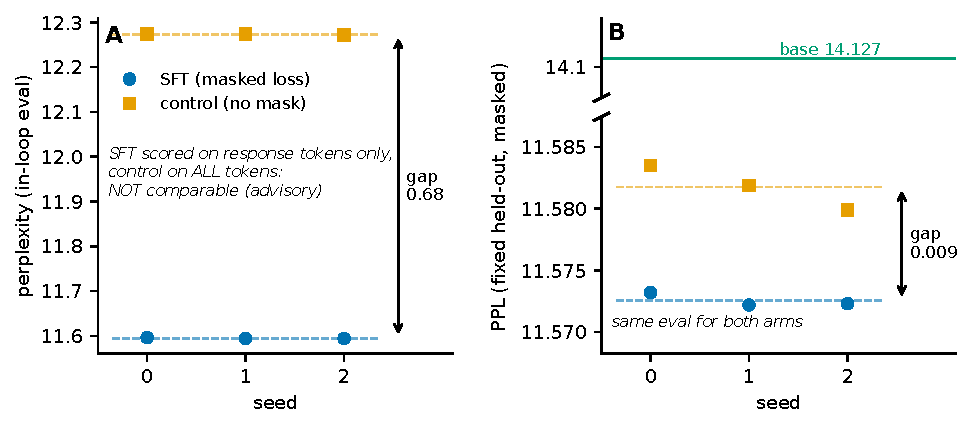
\includegraphics[width=0.9\linewidth]{figures/fig_sft_confound.pdf}
\caption{The SFT eval-token confound. Left: the in-loop advisory comparison
(training-loop perplexity, not suite-stamped) scores the SFT arm on response
tokens only and the control on all tokens, producing an incomparable
$+0.68$-PPL apparent gap (SFT 11.595 vs.\ control 12.273). Right: re-scored on
one fixed held-out response-masked set (66 OpenR1-Math documents, 228{,}529
response tokens, 13-gram dedup vs.\ train), the gap is $+0.009$ PPL (95\% CI
$[+0.0045, +0.0139]$) with a sign-flipping full-sequence cross-check
($-0.006$, n.s.) --- verdict directional. Budget: one pass over
125{,}000{,}592 OpenR1-Math tokens per arm, iso-FLOP, masking the only
variable; $n{=}3$ seeds per arm; across-seed spread SFT 0.001 / control 0.004
PPL. Source files: \texttt{verdict.json}, \texttt{reasoning\_verdict.json}
(2026-06-27 sft-3seed); rendered by \texttt{fig\_sft\_confound.py}.}
\label{fig:sft-confound}
\end{figure}
                 % 9. SFT vs iso-FLOP control + the eval-token de-confound
\section{RLVR at 0.6B: A Pre-Registered Null}\label{sec:rlvr}

The final lifecycle stage asks whether reinforcement learning from verifiable rewards (RLVR)
adds reasoning capability on top of the SFT checkpoint at this scale. The recent literature
motivates skepticism rather than optimism. \citet{yue2025does} argue that RLVR sharpens the
distribution the base model already supports---raising pass@1 while narrowing rather than
expanding pass@$k$ coverage---and \citet{shao2025spurious} show that Qwen-lineage models
improve under spurious and even random rewards, so an RLVR gain claimed on this lineage is
uninterpretable without a random-reward control. The stage plan (researched 2026-07-01, one
day before the 2026-07-02 launch) therefore pre-registered both the prediction and the
decision rule: on this FineWeb-Edu$\to$SFT base, which the plan characterizes as roughly
$10\times$ undertrained relative to compute-optimal token budgets \citep{hoffmann2022training},
RLVR is expected to sharpen rather than expand, ``the most likely true outcome is a
null-or-tiny attributable Dr.GRPO gain that the control battery should correctly refuse to
call a win,'' and a win may be declared only if GRPO beats \emph{both} the SFT floor and a
mandatory random-reward gate arm, with ``beats'' fixed in advance as non-overlapping Wilson
95\% confidence intervals.

\begin{figure}[t]
\centering
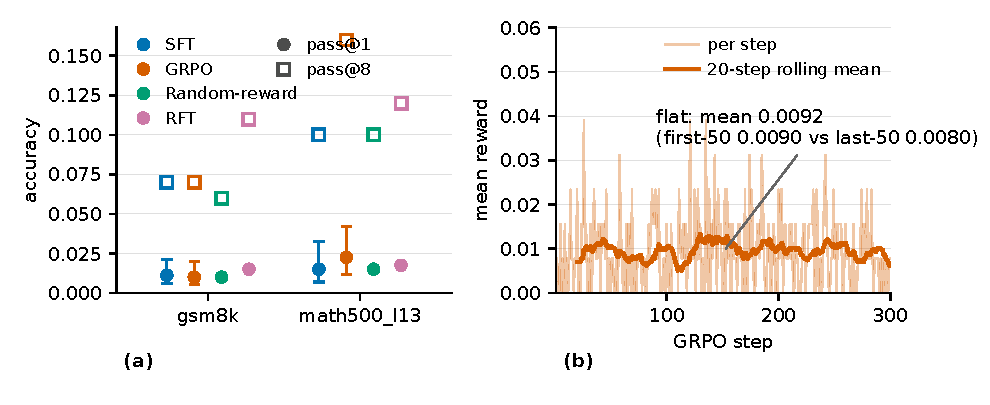
\includegraphics[width=\linewidth]{figures/fig_rlvr.pdf}
\caption{RLVR at 596M: pass@1 (Wilson 95\% CIs) and pass@8 \citep{chen2021evaluating} for the
SFT floor, Dr.GRPO, the random-reward gate arm, and the iso-generation-compute RFT control on
GSM8K (100 items) and MATH-500 levels 1--3 (50 items), 8 samples per item at $T{=}0.8$, band
seed 20260701, $n{=}1$ training seed, verifier pinned as \texttt{math-acc-v1}. GRPO trained
300 steps $\times$ 16 prompts $\times$ $G{=}8$ rollouts; its training reward stayed flat at
$\approx$0.9\% verifier-correct with no trend. All arm CIs overlap and both pre-registered
gates fail. Source files: \texttt{phase1\_passk.json}, \texttt{passk\_grpo.json},
\texttt{passk\_random.json}, \texttt{passk\_rft.json}, \texttt{health\_grpo\_seed0.jsonl}.}
\label{fig:rlvr}
\end{figure}

% tab_rlvr.tex -- RLVR Phase-2 paired eval: SFT floor / GRPO / random-reward gate / RFT control,
% on gsm8k (100 items) and math500_l13 (50 items), 8 samples each, plus the two pre-registered gates.
% Sources in Qwen3-0.6B/experiments/:
%   2026-07-01_qwen3-0.6b_rlvr-phase1-passk/phase1_passk.json (SFT + base cells, same band)
%   2026-07-02_qwen3-0.6b_grpo-phase2/passk_grpo.json, passk_random.json, passk_rft.json, verdict.json (gates)
\begin{table}[t]
\centering
\caption{RLVR at 596M: paired pass@$k$ of the SFT floor, Dr.GRPO, the random-reward (Spurious-Rewards) gate arm, and the iso-generation-compute RFT control, all decoded on the same band (100 GSM8K $+$ 50 MATH-500 level-1--3 items, 8 samples per item, $T{=}0.8$, max 256 new tokens, band seed 20260701; answer verifier pinned as \texttt{math-acc-v1}; both eval sets 0-flagged in a 13-gram decontamination check against the 35{,}924 SFT problems).
GRPO trained 300 steps $\times$ 16 prompts $\times$ $G{=}8$ rollouts; its training reward stayed flat at $\approx$0.9\% verifier-correct with no trend.
The RFT control collected 352 verifier-correct completions ($\approx$0.9\% of 38{,}400 rollouts) --- not 0, as an earlier draft misread from a smoke-test log line.
pass@1 carries a Wilson 95\% CI; pass@8 is the Chen et al.\ (2021) unbiased estimator; a gate ``passes'' only on non-overlapping Wilson CIs.
Both pre-registered gates FAIL on both sets, confirming the pre-registered null; RFT is nominally best on GSM8K (pass@8 11\% vs.\ 7\%) and GRPO on MATH-500 (16\% vs.\ 10\%), but all CIs overlap (n.s.), and GRPO's MATH-500 pass@1 merely ties the pretrain base (2.25\%).
$n{=}1$ seed, so the verdict is capped at \emph{directional}; phase 3 not launched.
Source files: \texttt{phase1\_passk.json} (SFT, base), \texttt{passk\_grpo.json}, \texttt{passk\_random.json}, \texttt{passk\_rft.json}, \texttt{verdict.json}.}
\label{tab:rlvr}
\footnotesize
\begin{tabular}{lcccc}
\toprule
 & \multicolumn{2}{c}{GSM8K (100 items)} & \multicolumn{2}{c}{MATH-500 L1--3 (50 items)} \\
\cmidrule(lr){2-3} \cmidrule(lr){4-5}
Arm & pass@1 \% (Wilson 95\%) & pass@8 \% & pass@1 \% (Wilson 95\%) & pass@8 \% \\
\midrule
SFT (floor)          & 1.12 $[0.59,\,2.12]$ & 7  & 1.50 $[0.69,\,3.23]$ & 10 \\
GRPO                 & 1.00 $[0.51,\,1.96]$ & 7  & 2.25 $[1.19,\,4.22]$ & 16 \\
Random reward (gate) & 1.00 $[0.51,\,1.96]$ & 6  & 1.50 $[0.69,\,3.23]$ & 10 \\
RFT (iso-gen.\ control) & 1.50 $[0.86,\,2.60]$ & 11 & 1.75 $[0.85,\,3.57]$ & 12 \\
\addlinespace
Base (reference, Phase 1) & 0.62 $[0.27,\,1.45]$ & 5 & 2.25 $[1.19,\,4.22]$ & 14 \\
\midrule
\multicolumn{5}{l}{\emph{Pre-registered gates (non-overlapping Wilson CIs required; outcome identical on both sets)}} \\
GRPO beats SFT floor    & \multicolumn{4}{c}{FAIL (\texttt{grpo\_beats\_sft\_floor} $=$ false)} \\
GRPO beats random gate  & \multicolumn{4}{c}{FAIL (\texttt{grpo\_beats\_random\_gate} $=$ false)} \\
\bottomrule
\end{tabular}
\end{table}


All arms are decoded on one fixed band: 100 GSM8K test items \citep{cobbe2021training} and 50
MATH-500 level-1--3 items \citep{hendrycks2021measuring}, 8 samples per item at temperature
0.8 with at most 256 new tokens, band seed 20260701. pass@1 carries a Wilson 95\% CI; pass@8
is the unbiased estimator of \citet{chen2021evaluating}; answers are scored by a pinned,
version-stamped verifier (math-acc-v1). Contamination was checked before any number was read:
a 13-gram index against the 35{,}924 SFT problems flags zero items in either eval set, and 14
eval-overlapping prompts were dropped from the GRPO training-prompt pool
(Table~\ref{tab:rlvr}).

A cheap Phase-1 gate preceded any RL spend. On this band (math-acc-v1) the SFT checkpoint
scores 1.1\% pass@1 on GSM8K (Wilson 95\% CI $[0.6, 2.1]$) and 7\% pass@8, and 1.5\%/10\% on
MATH-500 L1--3; the pretraining base scores 0.6\%/5\% and 2.25\%/14\% respectively
(Table~\ref{tab:rlvr}). The pre-registered GO rule was absolute solvability---proceed if and
only if the SFT arm solves at least 3 items across the band---and it fired with 12 solved
items. What the gate did \emph{not} establish should be stated plainly: GO fired on absolute
solvability, not on SFT beating the base. The SFT and base intervals overlap on every cell,
and the base beats SFT on MATH-500 pass@8 (14\% vs.\ 10\%)---an early warning that arm
separations near this accuracy floor sit inside the noise.

Phase 2 trained Dr.GRPO \citep{liu2025understanding} from the SFT checkpoint for 300 steps of
16 prompts $\times$ $G{=}8$ rollouts (38{,}400 rollouts total, at a measured $\approx$362~s
per step; roughly 88 hours estimated for the three arms): clip ratio 0.2, k3 KL penalty to the
frozen SFT reference with $\beta = 3\times10^{-3}$ (a coefficient flagged as inferred, not
paper-pinned), learning rate $10^{-6}$, and DAPO-style filtering of zero-variance rollout
groups \citep{yu2025dapo}, which retained 13.49 of 16 groups per step on average
(Table~\ref{tab:hparams})---the update was not gradient-starved. The training signal never
moved: the per-step verifier-correct rate (the fraction of the 128 rollouts per step scoring
exactly 1.0, not the shaped reward) is flat at $\approx$0.9\% (mean 0.0092; first-50-step
mean 0.009 vs.\ last-50 0.008; OLS slope $+5.8\times10^{-7}$ per step), and the per-token KL
to the reference stays near $1.7\times10^{-4}$ throughout, i.e., the policy barely moved
(Figure~\ref{fig:rlvr}). Two controls ran under the same recipe. The random-reward gate arm
\citep{shao2025spurious} replaced the verifier with a content-blind Bernoulli(0.5) draw and
trained at reward $\approx$0.5, confirming that the sampling, advantage, and update pipeline
all function. The RFT control spent iso-generation compute: it drew the same 38{,}400
rollouts, collected the 352 verifier-correct completions ($\approx$0.9\% of rollouts,
consistent with the GRPO reward floor), and ran one masked SFT pass over 200 of them.

Table~\ref{tab:rlvr} reports the final paired evaluation of all four arms on the same band
(math-acc-v1). On GSM8K, GRPO scores 1.0\% pass@1 / 7\% pass@8 against the SFT floor's
1.12\%/7\%, the random-reward arm's 1.0\%/6\%, and RFT's 1.5\%/11\%. On MATH-500 L1--3, GRPO's
nominal bump to 2.25\%/16\% over SFT's 1.5\%/10\% resembles the expected sharpening story
until it is compared with the pretraining base: GRPO's MATH-500 pass@1 of 2.25\% exactly
equals the base checkpoint's Phase-1 value on the same band, so the ``gain'' does not clear
the model the SFT stage started from. Both pre-registered gates fail on both eval sets: the
GRPO intervals overlap the SFT floor's and the random-reward gate's everywhere
(\texttt{grpo\_beats\_sft\_floor} and \texttt{grpo\_beats\_random\_gate} both evaluate to
false). The one nominally interesting cell---RFT's 11\% pass@8 on GSM8K against the floor's
7\%---is not significant (overlapping CIs) and, at one training seed, is at most a hypothesis
for future work.

The recorded verdict is \emph{directional}, capped by design rather than by accident: the
per-stage evaluation-completeness gate requires at least three paired seeds for any
non-directional RLVR call, and this cohort deliberately ran one seed with
proceed-to-phase-3 set to false---buying two further seeds would only have tightened a
confidence interval around zero. The pre-registered null is confirmed: at 0.6B, on this
undertrained base, the measurable reasoning gain arrived with SFT, not with RL, consistent
with the sharpen-not-expand account of \citet{yue2025does} and the Qwen-lineage
spurious-reward findings of \citet{shao2025spurious}. The claim is deliberately bounded. It
says nothing about RLVR at larger scales, on stronger bases, or with longer training; it says
that at this scale, under the controls the literature itself demands, an honest evaluation
battery refuses to call RLVR a win---and that a control battery designed before launch is
what makes such a refusal cheap.
                % 10. RLVR: pre-registered null (GRPO/random/RFT)
\section{What the Gates Caught: A Failure Catalogue}\label{sec:failures}

Every controlled result in this paper passed through the same mechanical gates: implausibility checks on scored verdicts, a fixed held-out evaluation set required before any win call, iso-FLOP confound checks, and a claim-to-file audit that opens every cited artifact. This section catalogues what those gates caught in the project's own work. Each entry gives the symptom, the detection mechanism, the root cause, the fix, and the guard that remains.

\paragraph{1. Token-level shuffle in the first data-mix run.}
Symptom: the 50/50 dclm-edu/FineWeb-Edu mix arm scored roughly $2\times$ \emph{worse} than both pure parents (wikitext-2 BPB 2.77 against $\approx$1.52, as recorded in the fix commit) -- physically implausible for a blend, whose loss should sit near the convex hull of its parents. Detection: the implausibility check on the verdict flagged it before any conclusion was recorded. Root cause: a \texttt{numpy} shuffle applied at the \emph{token} level interleaved the two sources token by token, destroying all sequence structure. Fix: commit \texttt{a576baa} concatenates the two coherent halves and mixes at the packed-sequence level, with the loader shuffling whole 4096-token windows. A 30-step probe after the fix shows the training cross-entropy descending from 11.65 to 8.04, where the token-soup variant had stayed flat near 11. The broken cohort was discarded and rerun; the corrected mix result appears in Table~\ref{tab:data}. Guard: the loader now carries an in-code warning, and the implausibility check stays in the scoring path.

\paragraph{2. The SFT eval-token confound.}
Symptom: in-loop advisory scoring showed response-masked SFT beating its iso-FLOP control by 0.68 perplexity, nominally significant (Figure~\ref{fig:sft-confound}; in-loop values, not suite-stamped). Detection: the protocol forbids a win call from in-loop numbers; a fixed held-out set must be scored first. Root cause: the SFT arm was scored on response tokens only while the control was scored on all tokens -- two incomparable token populations. On one fixed held-out response-masked set the gap collapses to $+0.009$ perplexity (95\% CI $[+0.0045, +0.0139]$, 3 seeds, paired), and a full-sequence cross-check gives $-0.006$ in the control's favor, not significant; the two disagree, so the verdict of record is directional (Section~\ref{sec:sft}, Table~\ref{tab:sft}). Guard: in-loop perplexities are permanently labeled advisory.

\paragraph{3. The RFT smoke-log misread.}
Symptom: an earlier draft of the RLVR verdict stated that the rejection-fine-tuning control collected zero verifier-correct completions. Detection: the claim-to-file audit for this paper re-read the full training log rather than its opening lines. Root cause: the ``0 collected'' line belongs to the one-step smoke test of 2026-07-02 at the top of the same log; the real 300-step run collected 352 of 38{,}400 rollouts ($\approx$0.9\%, matching the flat $\approx$0.9\% GRPO training reward; Table~\ref{tab:rlvr}). Fix: the verdict file and the repository README were corrected on 2026-07-06; the correction note is embedded in the regenerated artifact. The null verdict is unchanged -- 352 completions were too few to separate RFT from the floor -- but ``zero'' was wrong. Guard: smoke-test output is now read as a distinct log segment.

\paragraph{4. The README data-ratio pairing error.}
Symptom: repository documentation paired the $2.14\times$ gap-to-original with ``$\approx$275{,}000$\times$ less data.'' Detection: the claim-to-file audit; the source file pairs $275{,}000\times$ with the 131M-token Phase-A run, whose gap is $3.5\times$. Root cause: numbers from two different runs merged into one sentence. The correct pairing is $2.14\times$ at $\approx$30{,}000$\times$ less data (1.19B tokens) and $3.5\times$ at $\approx$275{,}000$\times$ less data (131M tokens), as in Figure~\ref{fig:repro-gap}; both gaps are ratios of in-loop validation perplexity, single run each, and are descriptive only. Corrected 2026-07-06.

\paragraph{5. The incomplete partial-RoPE-0.10 arm.}
The exploratory partial-RoPE-0.10 build died at step 5{,}450 of 18{,}150 ($\approx$30\% of budget), with a last-eval in-loop validation perplexity of 50.71 (single run, not suite-stamped). It is reported as incomplete in Section~\ref{sec:pretrain} rather than silently dropped -- an honesty entry rather than a gate catch.

\paragraph{6. A stale derived field in the ledger.}
Symptom: the ledger entry for the mid-training anneal carries a sub-field \texttt{c25\_cap} reading ``directional'' beside a verdict field reading ``win.'' Detection: the audit cross-checked every ledger field against the run's verdict artifact. Root cause: the cap predates the same-night upgrade that added the effective-context-length ladder and made the stage's required evaluation battery complete; the verdict fields were updated, the derived sub-field was not. The authoritative verdict file (no missing hard items) supports the win reported in Table~\ref{tab:midtrain}. Guard: noted as a standing hazard -- derived fields duplicated across artifacts can go stale independently of the record they summarize.

\paragraph{7. A parameter-count citation pointing at the wrong file.}
Symptom: the model README cited \texttt{verify.json} as evidence for the 596{,}049{,}920-parameter count (Table~\ref{tab:repro}), but that file contains no parameter field. The number itself is correct -- it is recovered exactly by recomputation from the architecture configuration and asserted in the build's test suite -- only the citation was off. Detection: the claim-to-file audit. Guard: every number in this paper traces to the file that actually contains it.

None of these seven was caught by re-reading prose. Each was caught by a mechanical gate: an implausibility check on a scored verdict, a fixed held-out set required before any win call, or a claim-to-file audit that opens every cited artifact. These are the same gates that validate the positive results of Sections \ref{sec:pretrain}--\ref{sec:rlvr}; a protocol that demonstrably catches its own errors is the strongest warrant this study can offer for the claims that survived it.
            % 11. What the gates caught (failure catalogue)
\section{Discussion}\label{sec:discussion}

\paragraph{What transfers.}
The portable output of this study is the evidence standard, not the effect
sizes. The unit of claim -- a paired across-seed bits-per-byte delta with a
95\% confidence interval on two corpora, under a single-variable diff at
matched train FLOPs, scored by a versioned suite (Section~\ref{sec:method})
-- is independent of scale and cheap relative to the training runs it
disciplines. Two empirical regularities also seem worth carrying forward.
First, bundle claims should be distrusted by default. The modernized bundle
\citep{grigorev2026imu} supplied this study's motivating headline, a 17.9\%
in-loop validation-perplexity gap at matched 1.19B-token compute (single
runs, in-loop, not suite-stamped; Table~\ref{tab:arms}); under
single-variable iso-FLOP re-tests it decomposed into three small,
individually significant architecture effects of +0.0256 to +0.0355 BPB on
wikitext-2 (each with a zero-excluding 95\% CI, 3 seeds, paired, 131M
tokens per cell, text-lm-v2), one large early-training optimizer-speed
effect (+0.4743 BPB, 95\% CI [+0.4435, +0.5052], 3 seeds, paired, 42M
tokens per cell), and two components -- the WSD schedule and z-loss -- that
contributed nothing measurable (Table~\ref{tab:attrib}). None of that
structure was visible in the bundle run. Second, data interventions
dominated at this scale. The largest attributed effect in the study is a
data swap: dclm-edu over FineWeb-Edu at +0.7034 code BPB (95\% CI
[+0.6639, +0.7430], 3 seeds, paired, 131M tokens per cell, text-lm-v2;
Table~\ref{tab:data}), and the mid-training anneal added +0.2716 code BPB
over its iso-token control (95\% CI [+0.2641, +0.2792], 3 seeds, paired,
150.7M tokens per cell, text-lm-v2; Table~\ref{tab:midtrain}). The
attributed architecture effects are an order of magnitude smaller
(Table~\ref{tab:attrib}), the optimizer effect is scoped to optimization
speed rather than converged quality, and the RL stage returned a
pre-registered null: GRPO beat neither the SFT floor nor the random-reward
gate, with training reward flat at $\approx$0.9\% (math-acc-v1, $n{=}1$
seed, directional by design; Table~\ref{tab:rlvr}, Figure~\ref{fig:rlvr}).
That null is consistent with the sharpen-not-expand reading of RLVR and
with documented spurious-reward effects on Qwen-lineage models
\citep{yue2025does, shao2025spurious} -- consistency, not confirmation,
given the single seed.

\paragraph{What does not transfer.}
The effect sizes themselves. Every comparison in this paper lives between
42M and 1.19B training tokens on one 596M-parameter architecture at
$\approx$2 tokens per parameter, far below compute-optimal
\citep{hoffmann2022training}. These are fixed-budget attributions; their
sign and size may change with budget, architecture, or data mixture, and
the paper makes no scale claim (Section~\ref{sec:limitations}).

\paragraph{The cost of rigor.}
Controls and seeds multiply compute. Computed from the recorded per-cell
budgets (Table~\ref{tab:attrib}), the de-confound ran 12 Phase-1 cells at
131,072,000 tokens each (1,572,864,000 tokens) plus nine Phase-2 cells at
the same budget (1,179,648,000 tokens): $\approx$2.75B training tokens,
roughly 2.3$\times$ the single 1.19B-token bundle run whose result they
re-attributed. That multiple is the price of replacing ``the bundle won''
with ``these components won, and these contributed nothing.'' Nulls cost
the same as wins: the SFT and RLVR stages spent full multi-arm budgets to
establish that nothing separable happened (Table~\ref{tab:sft},
Table~\ref{tab:rlvr}).

\paragraph{What an evidence-gated loop buys.}
The gates run even when no one is looking for a specific error. None of
the seven failures catalogued in Section~\ref{sec:failures} was caught by
re-reading prose; all were caught mechanically -- an implausibility check
on a blend scoring roughly twice the bits-per-byte of both its parents
(Table~\ref{tab:data}), a fixed held-out set that collapsed an in-loop
0.68-PPL ``win'' to +0.009 (Figure~\ref{fig:sft-confound}), and
claim-to-file audits that corrected two already-recorded claims (a
data-ratio pairing and a smoke-log misread) before writing. The same
machinery that catches the errors validates the positive results; the
discipline and the findings are one artifact.
          % 12. Discussion
\section{Limitations}\label{sec:limitations}

The gates of Section~\ref{sec:method} bound what this study can claim; this section states the limits that remain, each with its consequence.

\paragraph{Scale and regime.}
Every controlled effect was measured on a single 596{,}049{,}920-parameter architecture with a single tokenizer (151{,}936-entry vocabulary), at budgets between $\approx$42M and $\approx$1.19B tokens (Table~\ref{tab:arms}) -- all far below the compute-optimal regime for this size \citep{hoffmann2022training}. The attribution cells are early-training proxies (2{,}000 steps, $\approx$131M tokens per cell), and effects measured there may grow, shrink, or invert over longer horizons: every result is a fixed-budget attribution, never a scaling claim. The descriptive gap-to-original numbers -- a $2.14\times$ perplexity gap at $\approx$30{,}000$\times$ less data (1.19B tokens) and $3.5\times$ at $\approx$275{,}000$\times$ less data (131M tokens; Figure~\ref{fig:repro-gap}) -- are in-loop validation perplexities, single run each, not suite-stamped, and carry no interval.

\paragraph{Evaluation.}
``Bit-exact'' rests on a deterministic single-prompt fp32 forward comparison (Table~\ref{tab:repro}); it verifies the forward computation exactly under that protocol and nothing broader. The same SmolLM2 weights run on GPU show logit deltas of $4.72\times10^{-5}$ from kernel reduction-order differences (Table~\ref{tab:repro}), so exactness is a CPU-fp32 statement. The code corpus noise floor is $\approx$68\% of the measured value at the faithful baseline and reaches $\approx$92\% across the three build checkpoints (text-lm-v2; Table~\ref{tab:arms}), so code perplexity orderings are weakly powered and only the paired across-seed BPB intervals are relied on. BPB is measured on exactly two corpora -- wikitext-2 and Python code, both English-adjacent -- with no multilingual or broader-domain coverage. The SFT retention check on the standard suite used one representative seed per arm (Table~\ref{tab:sft}); its 3-seed intervals apply only to the in-domain reasoning set.

\paragraph{Statistics.}
Across all cohorts, seeds vary initialization and shuffle order over a fixed data split, so the reported intervals likely understate full-randomization variance. The off-anchor AdamW learning-rate points are single-seed, weight decay was held at 0.1 for both optimizer arms rather than tuned per arm, and the sweep bounds AdamW only within 1.7e-3 to 4.8e-3 (Table~\ref{tab:attrib}). The GRPO cohort has $n{=}1$ seed and is capped at directional by design (math-acc-v1; Table~\ref{tab:rlvr}). The passkey ladder uses $n{=}40$ probes per rung per cell, so individual rungs carry wide Wilson intervals (ecl-ladder-v1; Figure~\ref{fig:ecl-ladder}).

\paragraph{Unexplained observations.}
The base model's accuracy dip to 0.025 at its own 4{,}096-token trained window, repaired to 0.400 by both anneal arms (ecl-ladder-v1; Figure~\ref{fig:ecl-ladder}), has no defensible mechanism yet. The anneal's English improvement of $+0.0157$ BPB (95\% CI $[+0.0140, +0.0174]$, 3 seeds, paired, text-lm-v2; Table~\ref{tab:midtrain}) violated its pre-registered expected null and is reported as an exploratory observation, not a claim.

\paragraph{Hardware.}
All training ran on one GB10 workstation with $\approx$119 GB of unified memory. The device's peak throughput is an estimate, so any MFU figure is approximate and never quoted as exact, and no result has been replicated on other hardware or in a distributed setting.

These limitations are precisely why several repository-level verdicts remain directional rather than win: the data-composition records are capped by conservative bookkeeping (Table~\ref{tab:data}), the SFT record by a disagreeing full-sequence cross-check (Table~\ref{tab:sft}), and the RLVR record by its single seed (Table~\ref{tab:rlvr}). Under this protocol, a limitation that cannot be ruled out becomes a cap on the verdict -- which is the intended behavior.
         % 13. Limitations (REQUIRED)
\section{Reproducibility Statement}\label{sec:repro-statement}

All code, configurations, training and evaluation logs, decontamination
reports, and figure-generation scripts are public at
\url{https://github.com/yashb98/BuildFromScratch}. The entry point for any
replication is the verification gate: \texttt{cd Qwen3-0.6B \&\& python
verify.py} builds the model from the single-file implementation, loads the
published weights, and compares fp32 logits against the HuggingFace reference,
passing only if the maximum absolute logit difference is below the $10^{-3}$
tolerance with next-token argmax agreement; the recorded result is exactly
$0.0$ (Table~\ref{tab:repro}). The gate runs on CPU and needs no GPU.

Each experiment is isolated under
\texttt{Qwen3-0.6B/experiments/<RUN\_ID>/} and carries two machine-readable
artifacts: \texttt{c5\_evidence.json}, written before launch with the arm
plan, seeds, token budgets, and the iso-FLOP confound check, and
\texttt{verdict.json}, the scored outcome with per-seed values and confidence
intervals; runs are also recorded in a project ledger written only through
its programmatic interface (\texttt{research/ledger/ledger.py}). Every
quantitative value in this paper traces to a named on-disk file: the evidence
manifest that performs this mapping (\texttt{evidence\_manifest.json}) ships
with the paper source and lists, for each number, its source file and key or
line, including the mandatory caveats attached to each value.

All training ran on a single NVIDIA GB10 (Grace Blackwell) workstation with
$\approx$119~GB of unified CPU+GPU memory, using PyTorch with bfloat16 and
\texttt{torch.compile}; the 151,936-way cross-entropy is computed in chunks,
and every process caps its share of the unified pool before touching the
accelerator. Multi-seed comparisons use seeds 0/1/2
(Table~\ref{tab:hparams}). Cross-run comparable numbers come only from
versioned evaluation suites: text-lm-v2 (bits-per-byte and perplexity on
pinned corpus revisions, wikitext-2-raw-v1 at commit \texttt{b08601e0} and
codeparrot-clean-valid at commit \texttt{4db92d2e}), math-acc-v1 (a pinned
answer extractor and verifier), and ecl-ladder-v1 (the passkey context
ladder). In-loop trainer perplexities are labeled as such throughout and are
never compared against suite-stamped numbers. Thirteen-gram overlap
decontamination reports for the evaluation sets and prepared training sets
are stored on disk beside the corresponding datasets and results.
     % 14. Reproducibility (REQUIRED)
\section{Broader Impacts}\label{sec:impacts}

This is a small-scale measurement study conducted entirely on public
datasets: FineWeb-Edu \citep{penedo2024fineweb}, a DCLM-derived educational
subset \citep{li2024datacomp}, OpenR1-Math, GSM8K \citep{cobbe2021training},
and MATH \citep{hendrycks2021measuring}. It releases no new model capability:
the artifact is a 0.6B-scale reproduction of a published architecture
\citep{yang2025qwen3} trained on 1.19B tokens against the original's 36T
(Figure~\ref{fig:repro-gap}), and every recipe component studied is already
public.

The intended impact is methodological. Evidence-gated claims -- multi-seed
confidence intervals, iso-FLOP controls, versioned evaluation suites, and
pre-registered gates -- make small-model results cheaper to trust, and
publishing controlled negative results reduces wasted replication compute for
other resource-constrained groups. The SFT response-masking null
(Table~\ref{tab:sft}), the GRPO null at 0.6B (Table~\ref{tab:rlvr};
pre-registered, and reported as directional under the study's own single-seed
cap), and the context-extension stage gated off by a step-0 diagnostic are
reported in full rather than left in the file drawer; the RLVR arms carry a
content-blind random-reward control \citep{shao2025spurious} so that the null
is a measurement, not an absence of one.

The energy footprint is that of one desk-side workstation rather than a
cluster: a single machine ran every experiment, wall-clock time is recorded
per run in the shipped logs, and the largest single run -- the 1.19B-token
pretrain -- completed in 2663.1 minutes (per-stage budgets in
Table~\ref{tab:hparams}). Honest nulls at this scale are cheap to produce but
rarely published; reporting them alongside the study's two attributed wins is
the contribution this paper aims to make a norm.
     % 15. Broader impacts (REQUIRED)
\section{Conclusion}\label{sec:conclusion}

This paper reproduced Qwen3-0.6B to bit-exactness
($\max|\Delta\text{logits}| = 0.0$ under the recorded single-prompt fp32
protocol; Table~\ref{tab:repro}) and carried the reproduction through
pre-training, data composition, mid-training, supervised fine-tuning, and
RLVR under one evidence standard: single-variable diffs at matched train
FLOPs, three paired seeds, bits-per-byte confidence intervals on two
corpora, versioned eval suites, and pre-registration. Under that standard,
an $n{=}1$ bundle headline decomposed into three small attributed
architecture effects, an early-training optimizer-speed effect, and two
null components (Table~\ref{tab:attrib}); data interventions produced the
largest attributed effects (Tables~\ref{tab:data} and~\ref{tab:midtrain});
and three negative results -- response masking failing to separate from
its iso-FLOP control (Table~\ref{tab:sft}), a pre-registered GRPO null
reported as directional under the single-seed cap (Table~\ref{tab:rlvr}),
and context extension gated off at step 0 -- are reported to the same
standard as the wins, alongside a catalogue of the study's own corrected
errors (Section~\ref{sec:failures}). Two directions follow, stated as
directions only: measuring whether these fixed-budget effects persist as
the token budget grows toward compute-optimal, by re-running the same
single-variable ladders at increasing budgets; and a multi-seed RLVR
cohort, warranted only if a future base clears the Phase-1 solvability
floor decisively. Neither direction contributes any result to this paper.
          % 16. Conclusion

% ---- Bibliography ----------------------------------------------------
%  plainnat = numeric, sorted, natbib-compatible. arXiv AutoTeX does NOT
%  run BibTeX, so the tectonic-generated .bbl ships in arxiv_package.tar.gz
%  (refs.bib is included for provenance only; never hand-edit either).
\bibliographystyle{plainnat}
\bibliography{refs}

\end{document}
